\documentclass[a4paper,12pt,twoside,openany]{report}
%
% Wzorzec pracy dyplomowej
% J. Starzynski (jstar@iem.pw.edu.pl) na podstawie pracy dyplomowej
% mgr. inż. Błażeja Wincenciaka
% Wersja 0.1 - 8 października 2016
%
\usepackage{polski}
\usepackage{helvet}
\usepackage[T1]{fontenc}
\usepackage{anyfontsize}
\usepackage[utf8]{inputenc}
\usepackage[pdftex]{graphicx}
\usepackage{tabularx}
\usepackage{array}
%\usepackage[polish]{babel}
\usepackage{subfigure}
%\usepackage{amsfonts}
\usepackage{verbatim}
\usepackage{indentfirst}
\usepackage[pdftex]{hyperref}
\usepackage[none]{hyphenat}

%\usepackage{fancyhdr}
%\pagestyle{fancy}


\usepackage{subfigure}
%\usepackage{makeidx}

%\usepackage{floatrow}

%marginesy jakie są każdy widzi
\usepackage[tmargin=2cm, bmargin=1.8cm, lmargin=3.5cm, rmargin=2.0cm]{geometry}

%tytuły rozdziałów bez słowa "Rozdział"
%\usepackage{titlesec}
%\titleformat{\chapter}[display]{\normalfont\bfseries}{}{0pt}{\LARGE\thechapter.\ }
%\let\chaptername\relax


% rozmaite polecenia pomocnicze
% gdzie rysunki?
\newcommand{\ImgPath}{.}

% oznaczenie rzeczy do zrobienia/poprawienia
\newcommand{\TODO}{\textbf{TODO}}


% wyroznienie slow kluczowych
\newcommand{\tech}{\texttt}

% na oprawe (1.0cm - 0.7cm)*2 = 0.6cm
% na oprawe (1.1cm - 0.7cm)*2 = 0.8cm
%  oddsidemargin lewy margines na nieparzystych stronach
% evensidemargin lewy margines na parzystych stronach
%\def\oprawa{1.05cm}
%\addtolength{\oddsidemargin}{\oprawa}
%\addtolength{\evensidemargin}{-\oprawa}

%\geometry{tmargin=2cm, bmargin=1.5cm, lmargin=3.5cm, rmargin=2cm}

% table span multirows
\usepackage{multirow}
\usepackage{enumitem}	% enumitem.pdf
\setlist{listparindent=\parindent, parsep=\parskip} % potrzebuje enumitem

\renewcommand\labelitemi{--}

%%%%%%%%%%%%%%% Dodatkowe Pakiety %%%%%%%%%%%%%%%%%
\usepackage{prmag2017_bez_spisu}   % definiuje komendy opiekun, nrindeksu, rodzaj pracy, ...


%%%%%%%%%%%%%%% Strona Tytułowa %%%%%%%%%%%%%%%%%
% To trzeba wypelnic swoimi danymi
\title{Wpływ pracy zawodowej w ponadnormatywnym wymiarze czasu pracy na życie osobiste pielęgniarek i pielęgniarzy}

% autor
\author{Małgorzata Ługin-Dąbrowska}
\nrindeksu{3942}

\opiekun{dr n. med. Marta Gawlik}

\terminwykonania{1 maja 2022} % data na oświadczeniu o samodzielności
\rok{2022}

% Pielęgniarkom przyszłym i obecnym
%\podziekowania{\noindent
{\Large Podziękowania}
\bigskip

Dziękujemy bardzo serdecznie wszystkim, a w szczególności Rodzinom i~Unii Europejskiej...

\bigskip

{\raggedleft
Zdolny Student i Pracowity Kolega

}

}

\miasto{Legnica}
\uczelnia{Wyższa Szkoła Medyczna}
\wydzial{WYDZIAŁ PIELĘGNIARSTWA}
\kierunekstudiow{PIELĘGNIARSTWO}

% domyslnie praca jest inzynierska, ale po odkomentowaniu ponizszej linii zrobi sie magisterska
\pracamagisterska
%%% koniec od P.W

%\streszczenia{
%  \newpage
\begin{center}
\large \bf
TYTUŁ PRACY DYPLOMOWEJ
\end{center}

\section*{Streszczenie}
Praca składa się z krótkiego wstępu jasno i
wyczerpująco opisującego oraz uzasadniającego cel pracy, trzech rozdziałów (2-4)
zawierających opis istniejących podobnych
rozwiązań, komponentów rozpatrywanychjako kandydaci do
tworzonego systemu i wreszcie zagadnień wydajności wirtualnych
rozwiązań. Piąty rozdział to opis  środowiska obejmujący opis konfiguracji
środowiska oraz przykładowe ćwiczenia laboratoryjne. Ostatni
rozdział pracy to opis możliwości dalszego
rozwoju projektu. 

\bigskip
{\noindent\bf Słowa kluczowe:} praca dyplomowa, LaTeX, jakość

\vskip 2cm


\begin{center}
\large \bf
THESIS TITLE
\end{center}

\section*{Abstract}
This thesis presents a novel way of using a novel algorithm to solve complex
problems of filter design. In the first chapter the fundamentals of filter design
are presented. The second chapter describes an original algorithm invented by the
authors. Is is based on evolution strategy, but uses an original method of filter
description similar to artificial neural network. In the third chapter the implementation
of the algorithm in C programming language is presented. The fifth chapter contains results
of tests which prove high efficiency and enormous accuracy of the program. Finally some
posibilities of further development of the invented algoriths are proposed.

\bigskip
{\noindent\bf Keywords:} thesis, LaTeX, quality

\vfill
%}

%uaktywnić specjalne komendy związane z tworzeniem indeksów.
%\makeindex

\begin{document}
\sloppy
\maketitle

\end{document}

%\printindex


% Wykaz skrótów
\large Wykaz skrótów


\begin{table}[ht]
    
    \label{tab:index}
    %\begin{tabular}{*{2}{l}}
	\begin{tabular}{  l  l  }
	
	CBOS & Centrum Badania Opinii Społecznej\\

	Dz. U. & Dziennik Ustaw\\

	EBM & medycyna oparta na faktach (ang.: evidence-based medicine)\\

	MZ & Ministerstwo Zdrowia\\

	NIPIP & Naczelna Izba Pielęgniarek i Położnych\\

	OIPIP & Okręgowa Izba Pielęgniarek i Położnych\\

	POZ & Podstawowa Opieka Zdrowotna\\

	PTSD & zespół stresu pourazowego (ang.: post-traumatic stress disorder)\\

	SOZ & system ochrony zdrowia\\

	WHO & Światowa Organizacja Zdrowia (ang.: World Health Organization)\\

	ZNPZ & zespół nietolerancji pracy zmianowej \\

	
	\end{tabular}
   

\end{table}





%-----------------
% Wstęp
%-----------------

\chapter*{Wstęp}
... treść wstępu napiszę na końcu ...



%-----------------
% Wpływ pracy zawodowej pielęgniarek i pielęgniarzy na życie osobiste
%-----------------
\chapter{Wpływ pracy zawodowej pielęgniarek i~pielęgniarzy na życie osobiste w świetle literatury przedmiotu}
Zawód pielęgniarki należy do najbardziej prestiżowych profesji na świecie. W wydanym przez WHO i Międzynarodową Radę Pielęgniarek raporcie o stanie światowego pielęgniarstwa w roku 2020, podkreśla się szczególne znaczenie pielęgniarstwa, w każdym systemie ochrony zdrowia. Pielęgniarki pełnią kluczową rolę w sytuacji światowego zagrożenia zdrowotnego \cite{who}.  Również w Polsce coroczne rankingi najbardziej szanowanych zawodów, umieszczają tę grupę zawodową na wysokich pozycjach \cite{rap}. Mimo tego, od lat, obserwuje się znaczną dysproporcję między powszechną opinią o szacunku, a kojarzeniem zawodu z niskim wynagrodzeniem, ciężką pracą fizyczną i umysłową oraz nieustannymi wyrzeczeniami w życiu osobistym. Fenomen pogłębia fakt, iż pielęgniarki w większości, nie żałują wyboru zawodu, podkreślają, że daje  im wiele satysfakcji.

  %-----------------
  % Historyczne uwarunkowania samodzielności zawodowej.
  %-----------------
\section{Historyczne uwarunkowania samodzielności zawodowej}
Pielęgniarstwo ewaluowało na przestrzeni wieków, od spontanicznego odruchu serca, do autonomii wysokiego poziomu. Już w starożytności, nad cierpiącymi, czuwały osoby, wykonujące czynności pielęgnacyjne. Istnieją źródła historyczne, dotyczące organizacji opieki pielęgnacyjnej w starożytnych Indiach, Rzymie, Chinach, Japonii czy Grecji. Choć początkowo role te pełnili mężczyźni, to z czasem zawód stał się domeną kobiet \cite{zro}. Od czasów średniowiecza pielęgnowaniem chorych zajmowały się siostry zakonne. Tradycyjne zwracanie się do pielęgniarek ,,siostro”, tam ma, swój początek. Przez wiele wieków pielęgniarki, kojarzono ze złą reputacją \cite{tlo}. Fakt ten, związany był z zatrudnianiem do pielęgnowania chorych  osób z marginesu społecznego. Dopiero Florence Nightingale w połowie XIX w. pokonując liczne przeszkody, otworzyła szkołę dla pielęgniarek. Główny nacisk oprócz typowych umiejętności pielęgniarskich położono, na nienaganne zachowanie w pracy i poza nią. Jej działalność na rzecz podniesienia prestiżu zawodu, jest niepodważalna  \cite{flo}. Wychowała wiele pokoleń pielęgniarek. Jej uczennice niosły kaganek zmian, nawet na inne kontynenty. Przykładem może być Linda'e Richards, znana jako pierwsza wyszkolona pielęgniarka USA, która promowała pielęgniarstwo, również w Japonii \cite{linda}.

Niezwykle istotne, dla przyszłości światowego pielęgniarstwa, było utworzenie w Stanach Zjednoczonych Ameryki, na przełomie wieków, Międzynarodowej Rady Pielęgniarek \cite{rada}. Organizacji zrzeszającej profesjonalistów. Ściśle współpracującej z takimi instytucjami jak WHO, Czerwony Krzyż czy UNICEF. Choć pielęgniarki polskie, włączone zostały do jej struktur, dopiero 1948 roku, czynnie uczestniczyły w licznych projektach, dotyczących zdrowia i współpracy między tymi organizacjami.

W końcu nadszedł ten moment, w historii naszego zawodu, gdzie z poświęcenia i miłości bliźniego, przyszedł czas pielęgniarstwa zawodowego, opartego na wiedzy naukowej. Cytowane słowa, wybitnej pielęgniarki i nauczycielki Marii Minczewskiej, podkreślają znaczenie zawodu, u którego podstawy, leży  ochrona najważniejszych wartości ludzkich – życia i zdrowia.  Co zawarte jest w postulatach, takich ikon pielęgniarstwa jak Dorota Orem, Virginia Henderson, Madelaine Leininger \cite{ikon}.

Nie bez znaczenia dla jakości pielęgniarstwa, są kamienie milowe pionierek zawodu z Kanady – kształcenie na uczelniach wyższych, idee promocji zdrowia.

Podwaliny pod profesjonalny, prestiżowy zawód były solidne. I wydawać by się mogło, że pielęgniarstwo w Polsce, będzie się rozwijało, kwitło. Tak się nie stało. Na pewno wpływ na to miało położenie geopolityczne Polski. Sam fakt, że, przez ponad wiek kraj był pod zaborami, nie sprzyjał budowaniu tej istotnej dla państwa dziedziny. Wojny Światowe przerywały działalność szkół pielęgniarskich: lwowskiej, krakowskiej, warszawskiej, jednak pielęgniarki ratowały i pielęgnowały ludzi pod auspicjami Czerwonego Krzyża.

Najbardziej znane i zasłużone pionierki polskiego pielęgniarstwa rozumiały, że tylko nauka prowadzi do właściwego pełnienia tej roli zawodowej. Korzystały z kursów prowadzonych przez pielęgniarki Czerwonego Krzyża  w Polsce, wyjeżdżały za granicę. Miały otwarte umysły i chętnie dzieliły się wiedzą, tworzyły szkoły, uczyły.  Wyznawały pogląd, że żeby się dzielić, trzeba coś posiadać \cite{ikonpol}. I to, czyniły ze swoim potencjałem intelektualnym i materialnym. Wśród wielu, koniecznie wymienić trzeba Hannę Chrzanowską, Zofię Szlenkier, Elżbietę Rabowską, Annę Rydlównę. Pamiętać należy, w jak trudnych czasach przyszło im żyć, z jakim poświeceniem zdobywały wiedzę nie zważając na ostracyzm, przeciwności losu. Tym bardziej, te przykłady powinny inspirować do świadomego wyboru i wykonywania zawodu pielęgniarki. Cieszy fakt, że ich rola była doceniana nagrodami np. medalem Florence NIghitngale, stypendiami np. Fundacji Rockefellera \cite{50}.

Po II Wojnie Światowej powrócono do kształcenia w zawodzie pielęgniarki. Nauka była prowadzona przez szkoły świeckie, pomaturalne. Istniały także krótkie ścieżki zawodowe. Powstała szkoła dla instruktorek pielęgniarstwa.

W kolejnych latach pojawiały się branżowe magazyny: Pielęgniarka Polska, Położna, a w efekcie połączenia tych periodyków w 1958 roku, Pielęgniarka i Położna. Wydawane przez Polskie Towarzystwo Pielęgniarskie \cite{czas}.

W 1968 roku Ministerstwo Zdrowia przyjęło zaproponowany system wyodrębnionych dziedzin pielęgniarskich. I tak pojawiło się pielęgniarstwo pediatryczne, psychiatryczne, zachowawcze, środowiskowe, operacyjne i chirurgiczne. Szkolenie w tych kierunkach prowadzone było w systemach stacjonarnych i zaocznych i trwało dwa lata. W 1971 roku w Lublinie pierwsze pielęgniarki mogły się kształcić również, w ramach studiów dziennych na Akademii Medycznej. Kolejne uczelnie medyczne otworzyły swoje podwoje dla tego kierunku wkrótce po tym \cite{spec}.
 
Od 2007 roku, aby zostać pielęgniarką, nie wystarczy ukończyć Liceum czy Studium Medycznego. Należy podjąć studia na Uniwersytetach Medycznych lub Wyższych Uczelniach Zawodowych, w celu zdobycia tytułu zawodowego Licencjata czy Magistra Pielęgniarstwa. Samorząd Zawodowy Pielęgniarek i Położnych umożliwił osobom wykształconym w poprzednim systemie nauczania tzw. studia pomostowe, po ukończeniu, których absolwent otrzyma tytuł zawodowy Licencjata Pielęgniarstwa oraz możliwość zdobycia kolejnego tytułu zawodowego – Magistra Pielęgniarstwa \cite{model}.

  %-----------------
  % Ustawa o zawodzie pielęgniarki i położnej pierwszym krokiem do autonomii zawodu.
  %-----------------
\section{Ustawa o zawodzie pielęgniarki i położnej pierwszym krokiem do autonomii zawodu}
Determinantami każdego niezależnego zawodu, są: regulacje prawne i organizacyjne, wiedza, doświadczenie, autorytet, profesjonalizm i określony system wartości \cite{deter}.

Pierwsze zalążki rodzącej się autonomii zawodowej pojawiają się jeszcze przed II Wojną Światową. Długofalowe działania na rzecz ustawodawstwa są zasługą pielęgniarek m.in.  Marii Babickiej- Zachert, Heleny Nagórskiej, Zofii Zawadzkiej, Elżbiety Rabowskiej, Zofii Szlekier piastujących kierownictwa Referatu Pielęgniarstwa w Departamencie Zdrowia kierownictwa szkół pielęgniarskich, szkół PCK i wielu innych wybitnych postaci ze środowiska medycznego.

Ustawa ostatecznie weszła w życie w lipcu 1935 roku \cite{usta}. Stanowiła akt ramowy. Dający ogólne wytyczne i ustalenia najważniejszych kwestii. Mimo, to sam fakt jej uchwalenia był dowodem na rangę zawodu, wysoką ocenę społeczną i państwową. Była wykładnikiem dążeń do podniesienia jakości polskiego pielęgniarstwa. Z chwilą wejścia w życie, zmniejszyła się liczba osób niedostatecznie wykwalifikowanych w zawodzie. Stworzono dla nich okresy przejściowe, warunki otrzymania uprawnień. Pielęgniarki zyskały ochronę swoich praw zawodowych. Wprowadzono rejestr, w celu ewidencji, racjonalnego zarządzania kadrą, nakaz okazania świadectwa zdrowia, zagadnienie tajemnicy zawodowej. Na uwagę zasługuje fakt, iż pielęgniarki zaliczono do pracowników umysłowych. Ustawa zawierała wytyczne dotyczące szkół pielęgniarskich, symboli, umundurowania, a także postanowienia karne \cite{1935}.

Ustawą, która trwale zmieniła postrzeganie zawodu pielęgniarki jako zawodu wykonawczego dla kadry lekarskiej, jest ustawa o zawodach pielęgniarki i położnej z 1996 roku \cite{1996}. Już na początku aktu normatywnego wyraźnie podkreśla, że zawody pielęgniarki i położnej, są samodzielnymi zawodami medycznymi. Rodzi to określone konsekwencje. Pielęgniarka posiada niezależność podczas realizacji zadań, tzn. planuje pracę własną, dobiera metody pracy, dokonuje ewaluacji. Równocześnie podejmując decyzje, ponosi za nie, odpowiedzialność. To osoba pracująca z zespołem terapeutycznym, a nie dla lekarza. Ukierunkowana na pacjenta, a nie na jego chorobę. Aby móc sprostać tym wymaganiom ustawa daje jasne wskazówki dotyczące drogi zawodowej, konieczności ustawicznego kształcenia. Dodatkowo ustawa daje możliwość do realizowania się jako pielęgniarka, na stanowiskach nie, stricte pielęgniarskich np. związanych z procesem edukacji, administrowaniem w placówkach ochrony zdrowia, podmiotach typu żłobek, dom pomocy społecznej, czy pełnieniem funkcji w samorządzie zawodowym i związkach zawodowych.

Wszystkie zagadnienia tej ustawy były niezwykle ważne, choć w dużej mierze ogólnikowe. Kolejna ustawa z 2011 roku w swoich 104 artykułach, jest już bardziej precyzyjna we wszystkich kwestiach. Zwiększyła się liczba potencjalnych instytucji, w których pielęgniarka mogłaby być zatrudniona, bez ryzyka utraty prawa zawodu np., pełnienie służby na stanowiskach służbowych w Ministerstwie Obrony Narodowej, na których wykonuje się czynności związane z ochroną zdrowia i opieką zdrowotną, podobnie w więziennictwie, instytucjach samorządowych \cite{2011}. 

Na rangę zawodu wpływa posiadanie własnego organu usankcjonowanego prawnie. W przypadku pielęgniarek i położnych jest to samorząd zawodowy. W jego skład wchodzą Naczelna Izba Pielęgniarek i Położnych z siedzibą w Warszawie, oraz okręgowe izby pielęgniarek i położnych z siedzibami w miastach wojewódzkich. Statut organizacji, jej zadania zawarte są w ustawie z dnia 1 lipca 2011 roku o samorządzie pielęgniarek i położnych. Samorząd tworzą pielęgniarki/arze i położne/i posiadający czynne prawo wykonywania zawodu i wpisani do rejestru danej Izby Pielęgniarskiej. Przynależność do samorządu jest obowiązkowa dla wszystkich zarejestrowanych. Przedstawiciele wybierani są na okres 4 lat. Ich zadaniem jest reprezentowanie środowiska pielęgniarskiego i położniczego, w szczególności sprawowanie pieczy nad należytym wykonywaniem zawodu poprzez przyznawanie prawa wykonywania zawodu i pociąganie do odpowiedzialności zawodowej swych członków \cite{nipip}.

Narastające stale tempo życia, stres, postęp technologiczny, nadmierne eksploatowanie surowców naturalnych oraz wydłużenie życia ludzi prowadzi do nieuniknionych zmian. Dlatego rośnie rola zawodów medycznych, w tym pielęgniarki. Następuje przesunięcie zadań z chorób, na promocję zdrowia, co wyraża się usystematyzowaniem pełnionych przez pielęgniarkę funkcji :
\begin{itemize}
	\item zapewnia swoją pomoc, stosownie do potrzeb i problemów zdrowotnych człowieka, rodziny, grup społecznych w zakresie promowania zdrowia, zapobiegania chorobom i przywracania zdrowia, uczy i oddziałuje wychowawczo, wspiera, pomaga, organizuje, kieruje, zastępuje;
	\item kształtuje współpracę z człowiekiem, z ludźmi, którym zapewnia swoją pomoc;
	\item podejmuje działania na rzecz ciągłego podnoszenia jakości i efektywności pielęgnowania.
\end{itemize}

Wraz z rosnącą samodzielnością pielęgniarki zostały objęte ustawową ochroną przewidzianą dla funkcjonariuszy publicznych \cite{prawo}. Przepisy mają za zadanie chronić godność i nietykalność cielesną pielęgniarek i położnych, w związku z pełnieniem przez nie obowiązków zawodowych. To jest niezwykle istotne, w świetle coraz częściej występujących incydentów agresji słownej i fizycznej.

Samodzielność zawodowa sukcesywnie ewoluuje dzięki kolejnym Rozporządzeniom Ministra Zdrowia \cite{akty}:
\begin{itemize}
	\item w sprawie recept wystawianych przez pielęgniarki i położne;
	\item w sprawie rodzaju i zakresu świadczeń udzielanych przez pielęgniarkę, albo położną samodzielnie bez zlecenia lekarskiego;
	\item w sprawie wykazu substancji czynnych zawartych w lekach, środków spożywczych specjalnego przeznaczenia żywieniowego i wyrobów medycznych ordynowanych przez pielęgniarki i położne oraz wykazu badań diagnostycznych, na które mają prawo wystawić skierowania pielęgniarki i położne;
	\item w sprawie świadczeń gwarantowanych z zakresu ambulatoryjnej opieki specjalistycznej. Dotyczące porady pielęgniarskiej w AOS i POZ.
\end{itemize}

Wszystkie te możliwości prawne zwiększają autonomię i niezależność pielęgniarek. Mogą one, bez zlecenia lekarskiego wykonywać świadczenia profilaktyczne, diagnostyczne, lecznicze i rehabilitacyjne. Samodzielnie ordynować leki i wyroby medyczne. Wypisywać recepty, po uzyskaniu specyficznych uprawnień i kompetencji. Liczba procedur i kompetencji pielęgniarskich wzrasta proporcjonalnie do potrzeb zdrowotnych. Widoczne jest to, szczególnie teraz, gdy istnieje realne zagrożenie epidemiczne rozprzestrzeniającym się i stale mutującym wirusem SarsCov 2. Na mocy kolejnych rozporządzeń pielęgniarki kwalifikują do szczepień, udzielają teleporad, wykonują badania fizykalne.

Przyjęta przez Radę Ministrów strategia dotycząca rozwoju pielęgniarstwa i położnictwa w Polsce   w październiku 2019 roku, zawiera ambitne plany zwiększenia liczby pielęgniarek i położnych, powstrzymanie emigracji zarobkowej, zmotywowanie absolwentów szkół średnich do podejmowania studiów pielęgniarskich i kariery w zawodzie, utrzymanie na rynku pracy pielęgniarek i położnych, w tym nabywających uprawnienia emerytalne. Te działania planowane są na najbliższe 15 lat i będą weryfikowane co 5 lat \cite{strategia}.

Niezależność, samodzielność zawodową uważa się za kluczowy czynnik rozwoju, a zarazem motywację do pracy. Autonomia decyduje o satysfakcji zawodowej, a jej brak skutkuje mniejszym zaangażowaniem. Fedreric Laloux przekonuje, że ludzie najlepiej pracują w warunkach wolności, partnerstwa, zaufania i współpracy. W takich warunkach, są kreatywni, zmotywowani i efektywni. Nie ma potrzeby ich kontrolować. Nie podejmują nieprzemyślanych decyzji, konsultują swoje pomysły z członkami zespołu i dzięki zaufaniu, którym są obdarzani stają się odpowiedzialni za własne działania \cite{federic}. Takie mogą i powinny być pielęgniarki. Ale czy pielęgniarki są otwarte na nowoczesne pielęgniarstwo? Pielęgniarstwo na światowym poziomie, poparte dowodami naukowymi? Czy raczej zmęczone świadczeniem usług pielęgniarskich w kilku placówkach, dbaniem o mir domowy, nie są zainteresowane niezależnością zawodową, popartą wiedzą i kompetencjami? Przedstawicielki zawodu w Polsce uważają, że potrzebna będzie przebudowa mentalna, ale te zmiany są wartościowe i potrzebne dla obecnych i przyszłych pokoleń pielęgniarek. Pozytywne zmiany odczują także pacjenci, a to jest sedno pielęgniarstwa.

  %-----------------
  % Kompetencje i uprawnienia zawodowe pielęgniarek i pielęgniarzy.
  %-----------------
\section{Kompetencje i uprawnienia zawodowe \newline pielęgniarek i pielęgniarzy}
Pielęgniarstwo w Polsce, nigdy nie było profesją, w którą inwestowaliby rządzący, niezależnie jaką opcję polityczną by reprezentowali. Wszystkie osiągnięcia zawdzięcza ciężkiej pracy swych przedstawicielek oraz licznych grup pielęgniarek i pielęgniarzy organizujących marsze, strajki, monitujących pielęgniarek- posłanek w Sejmie, roboczych grupach komisji zdrowia. Nigdy nie postawiły one na szali, życia i zdrowia pacjenta \cite{strajk}. Mimo tego, że zawód, jest trudny i w porównaniu z innymi profesjami nie jest atrakcyjny pod względem finansowym, funkcjonujące w systemie pielęgniarki spełniają wymogi ustawy o zawodzie pielęgniarki i położnej  w zakresie ustawicznego kształcenia \cite{2011}. Łącznie liczba pielęgniarek i położnych posiadających tytuł licencjata i magistra pielęgniarstwa, oraz tytuł licencjata i magistra położnictwa to połowa zarejestrowanych aktywnych zawodowo pielęgniarek i położnych \cite{ile}. Pielęgniarki w Polsce podejmują również studia doktoranckie, prowadzą badania oparte na dowodach naukowych EBM, są cenionymi naukowcami w strukturach światowych organizacji. Polskie pielęgniarki są kreatywne, otrzymują wyróżnienia, nagrody. W 2021 roku Nagrodę Pielęgniarską Królowej Szwecji Queen Silvia Nursing Award zdobyła Julia Osiecka, za projekt- powrót do młodych lat. Laureatka zachęca do wykorzystania wirtualnej rzeczywistości do przedstawienia i doświadczania aktywności, które w młodości były codziennością obecnych seniorów \cite{julia}. Wszystkie propozycje zgłoszone do nagrody były innowacyjne i warte rozwoju. Nie promuje się jednak  pielęgniarstwa i nie pomaga w tym narracja w mediach - seriale fabularne i paradokumenty fałszują obraz pielęgniarki \cite{postrzeganie}.

Kompetencje, to ranga, nobilitacja, ale również odpowiedzialność i nierozerwalnie z nią związane roszczenia pacjentów. Środowisko pielęgniarskie, boi się konsekwencji i niechętnie korzysta ze swoich uprawnień. Widać to szczególnie w ilości wystawianych recept przez uprawnione pielęgniarki. W pierwszej połowie 2019 roku receptę wystawiło 2150 pielęgniarek \cite{model}. Za przyczyny tego faktu podaje się brak wymogów formalnych, dynamiczny system refundacji leków, trudności proceduralne takie jak dostęp do systemu E-wuś, podpis certyfikowany, zakładanie konta na platformie P1, konieczne jest zaplecze sprzętowe, spełniające określone wymagania techniczne.  Nie bez znaczenia jest także odpowiedzialność, także finansowa. Poza tym za nowymi kompetencjami, czyli kolejnymi obowiązkami, nie następuje wzrost wynagrodzeń za usługę. Niewykorzystana szansa systemu, gdzie w czasach zagrożenia epidemicznego, pacjenci muszą się narażać pobytem w placówce ochrony zdrowia, w celu wypisania czy przedłużenia recepty. Podobne dylematy dotyczą pozostałych nabytych kompetencji pielęgniarskich. Rzeczywiste wykonywanie tych czynności zmieniłoby postrzeganie pielęgniarki przez społeczeństwo jako służącej pana doktora, na korzyść pielęgniarki profesjonalistki, która z powodzeniem dokona badania fizykalnego, zleci i dokona analizy badań i jeśli będzie to konieczne zaordynuje odpowiednie leki. Profesjonalizm przekłada się na prestiż, którego wykładnią są adekwatne wynagrodzenia. 

To wszystko budzi frustrację i nie sprzyja homeostazie zawodowo rodzinnej.  Te same bariery dotyczą badań fizykalnych w codziennej praktyce pielęgniarskiej. Niewiele  pielęgniarek  korzystających ze stetoskopu,  można spotkać na oddziałach. I mimo, iż badania fizykalne są przedmiotem w programie edukacji studiów pielęgniarskich, przystąpienie do szkolenia specjalizacyjnego z danej dziedziny wymaga świadectwa ukończenia wyżej wymienionego kursu, to nie przekłada się to na pracę zawodową. W literaturze zagadnienia dotyczącego skali światowej, podkreśla się, że sytuacja jest lepsza w krajach, gdzie na oddziałach szpitalnych jest mniejsza liczba lekarzy, specjalistów. To brak kadry lekarskiej spowodował przesunięcie tego rodzaju kompetencji na pielęgniarki. Badaniem fizykalnym w pełnym zakresie zarówno manualnym i sprzętowym posługują się tam pielęgniarki pielęgniarstwa zachowawczego, kardiologiczne, nefrologiczne, anestezjologiczne i dializacyjne. W mniejszym stopniu ze swoich uprawnień korzystają pielęgniarki innych specjalności \cite{badania}.W Polsce niestety nie mamy się czym chwalić w tym zakresie, chociaż pojawiają się pionierzy, w postaci pielęgniarzy młodego pokolenia, którzy widzą w tym szansę na rozwój, prestiż. Chętnie o tym mówią i propagują nowoczesne pielęgniarstwo. Prowadzą oni swoje blogi, podkasty, strony internetowe, a co najważniejsze propagują treści zgodne z aktualną wiedzą.  Pokazują rzeczywistość, szukają rozwiązań, zapraszają gości, którzy dzielą się swoją wiedzą i poszerzają horyzonty przepracowanych pielęgniarek, promują pielęgniarstwo \cite{spoty}.

Niewykorzystanie  kompetencji, jest ogromną stratą dla pielęgniarstwa, dla pacjenta. Powszechnie wiadomo, że zaciera się granica między pielęgniarstwem, a medycyną. Ukierunkowanie działań medycznych już od dawna zmierza, ku holizmowi. Aspekt biopsychospołeczny jest podstawą w indywidualnym planie opieki pielęgniarskiej \cite{dorota}. Piękne założenia, idee, ale rzeczywistość pielęgniarek jest trudna. Oprócz oczywistych powodów jak wynagrodzenie wynikające z dodatkowych kompetencji, obserwuje się jeszcze niechęć środowiska lekarskiego oraz mniejsze zaufanie pacjentów, do pielęgniarek wykorzystujących nowe uprawnienia. Mimo to pielęgniarki rozumieją ideę i konieczność zmiany systemu i  pojawiające się możliwości, co obrazują petycje kierowane do Naczelnej Izby Pielęgniarek i Położnych w sprawie poszerzenia kompetencji dla grupy zawodowej magistrów, licencjatów i specjalistów pielęgniarstwa i położnictwa \cite{petycja}. Współpraca w ramach zespołu do zmian w podstawowej opiece zdrowotnej POZ, przy Ministrze Zdrowia również świadczy o powadze zawodu i prestiżu \cite{poz}.

  %-----------------
  % Zdrowie pielęgniarek
  %-----------------
\section{Zdrowie pielęgniarek}
\label{sectionZdrowiePielegniarek}
Do czynników wpływających na stan zdrowia pielęgniarek należą ogólne warunki pracy, zasoby ludzkie i materiałowe, organizacja czasu pracy,  praca zmianowa, ale także fizyczne czynniki środowiskowe: temperatura, wilgotność, ruch powietrza, hałas, oświetlenie, promieniowanie jonizujące, materiał biologiczny czy substancje chemiczne. Znaczenie ma także tzw. kultura organizacji, stosunki panujące wewnątrz niej, rodzaj, specyfika i natężenie pracy \cite{obciazenia}.

Ostatnie badania na temat długości życia kobiet w Polsce jasno pokazują, że długość życia pielęgniarek jest zdecydowanie krótsza, niż średnia kobiet i sukcesywnie się zmniejsza. I tak w według danych Naczelnej Izby Pielęgniarek i Położnych przeciętna długość życia pielęgniarek w Polsce wynosiła w 2020 roku 63,8 lat, przy przeciętnym wieku kobiet w Polsce 81.8 lat. Łączna średnia z lat 2016-2020 jest jeszcze niższa i wynosi 61,4 lata \cite{statystyka}.

W roku 2021 umieralność wśród pielęgniarek wyniosła aż 1,6 tysiąca pielęgniarek. Prezes Naczelnej Izby Pielęgniarek i Położnych uzasadnia, iż jest to wynikiem ciężkiej pracy zmianowej, bez odpowiedniej ilości odpoczynku, regeneracji. Pielęgniarka z 25 letnim stażem, pracująca na nocne zmiany nie przespała we własnym łóżku w domu pięciu lat. To musi się odbić na zdrowiu fizycznym, psychicznym, funkcjonowaniu psychospołecznym. Zmęczenie, bezsenność, zwiększenie ryzyka urazów i wypadków, brak kontaktów towarzyskich, aktywności fizycznej innej niż zawodowa, kłopoty z pamięcią, trudności w uczeniu się, liczne choroby, zwiększone ryzyka nagłych stanów \cite{zgony}.

Pandemia Covid 19 miała kolosalny wpływ na wzrost występowania zaburzeń snu, wśród pracowników ochrony zdrowia. Połączenie stresu i deprywacji snu stanowi ryzyko myśli samobójczych, depresji i ogólnie pojętej złej jakości życia, było przedmiotem badań pielęgniarek w szpitalach w Ottawie. Wyniki badań są istotnie znaczące klinicznie. Grupa zostanie  zbadana ponownie  po zakończeniu pandemii \cite{sen}.

Te przygnębiające statystki pogłębia fakt, że z każdym rokiem coraz więcej pielęgniarek odchodzi na emerytury. Wiele z nich zmuszonych jest pracować nadal, głównie ze względów finansowych.  Największy liczbowo przedział wiekowy tej grupy zawodowej to 51-60 lat. Co stanowi blisko 36\% ogólnej liczby wszystkich przedstawicieli zawodu. Nowy dopływ personelu pielęgniarskiego, nie jest wystarczający, by zabezpieczyć w pełni etaty w placówkach świadczących usługi zdrowotne. Co oznacza, że pracujące wciąż w systemie pielęgniarki, dźwigają ciężar opieki nad pacjentem na swoich barkach nie rzadko ponad dobę, wypracowując nawet 300 godzin miesięcznie. Osoby, które podejmują dodatkową pracę, wykonują niejako pracę od 1,5 do 2,6 etatu \cite{cyfrowe}. Aby to zobrazować, podaje się przykład, gdzie w wyniku zaprzestania pracy dodatkowej oraz zaprzestania pracy przez emerytowane pielęgniarki dochodzi do zamknięcia kilkudziesięciu szpitali w Polsce. W samym województwie Kujawsko-Pomorskim 11. Raport NIPP dotyczący sytuacji kadrowej w zawodzie podkreśla, brak zastępowalności pokoleń w zawodzie \cite{statystyka}. Ciężar pracy wykonywanej ponad normę ma ścisłe odzwierciedlenie w  stanie psychicznym,jakości  odpoczynku, relacjach międzyludzkich – tak ważnych w komunikacji z pacjentem, członkami zespołu terapeutycznego. Jak to odbija się na powierzanych zadaniach? Za błąd ludzki ceną jest życie człowieka – pacjenta, jego rodziny jak również pielęgniarki i jej bliskich. Jak można edukować, promować zdrowie, kiedy samemu się nie jest wzorem do naśladowania? Czy to przejaw hipokryzji, czy po prostu życiowa konieczność? Takie pytania powinny sobie postawić pielęgniarki i pielęgniarze czynni zawodowo.

W literaturze przedmiotu obciążenia stanowiska pracy określa się stopniem zaangażowania pracownika w wykonywaną pracę lub liczbą występujących skutków tego zaangażowania \cite{stanowisko}. Tym czasem realia w polskich jednostkach zdrowia, nie zostawiają najmniejszych złudzeń w tym względzie. Praktyka jest odległa od teorii, a przeciążony pracą personel nie jest skuteczny w działaniu, popełnia błędy, nie jest empatyczny w stosunku do chorych i koleżanek, kolegów. Prowadzi to, do konfliktów, złej atmosfery w pracy, co przekłada się na zaburzenia, snu, opóźnia procesy myślowe, wywołuje objawy somatyczne takie jak bóle głowy, nudności, bóle brzucha, biegunki czy zaparcia. Pojawiają się choroby przewlekłe takie jak depresja, cukrzyca, choroby autoimmunologiczne \cite{zdrowie}.

Wszechobecny stres i brak możliwości użycia wentyli bezpieczeństwa, występujące zjawisko wtórnej traumatyzacji oraz zespól stresu pourazowego sprzyja chorobom nowotworowym i i układu krążenia \cite{skutki}. Natomiast deficyty w stosowaniu zbilansowanej, wartościowej diety, nadużywanie używek: kawa, napoje energetyczne, nierzadko środki pobudzające prowadzą do chorób układu pokarmowego \cite{p.p}. Przeciążenia wynikające z niestosowania się do przepisów BHP w zakresie podnoszenia, przesuwania skutkują chorobami układu ruchu, obniżeniem narządów miednicy i kolejnymi niekorzystnymi zmianami. Co znamienne większość chorób występujących w Wykazie Chorób Zawodowych dotyczy personelu medycznego \cite{wykaz}. Faktyczny obraz współczesnej polskiej pielęgniarki odbiega znacznie od tych, które prezentowane są w zagranicznych serialach telewizyjnych i niestety mijają się z profesjonalizmem, do którego osoby pracujące w zawodzie pretendują.

Jednak mimo krytycznej sytuacji w Systemie Ochrony Zdrowia istnieją narzędzia, które można i należy wykorzystać dla zachowania własnego zdrowia. Jednym z nich jest poczucie własnej skuteczności \cite{skutecznosc}. Ma ono szczególne znaczenie dla pielęgniarek i pielęgniarzy czynnych zawodowo. Ponieważ im wyższe poczucie własnej sprawczości, zaradności i skuteczności, tym wyższa homeostaza emocjonalna, łatwość w radzeniu sobie w sytuacjach stresujących\cite{salutogeneza}. Poczucie własnej skuteczności jest swoistym płaszczem ochronnym, gdyż zapobiega wypaleniu zawodowemu. To umiejętność, która polega na pozytywnym podejściu do stresu (jako czynnika rozwoju, motywacji), rozumieniu mechanizmu stresu, sposobów niwelowania napięć. Wymaga zatem pogłębiania wiedzy, treningu i praktyki. Ostatecznie przekłada się na wysoką odporność psychiczną, zdrowie, zaradność, efektywność w działaniu, a w rezultacie profesjonalizm i wzrost opieki pielęgniarskiej \cite{stres}.

  %-----------------
  % Życie osobiste pielęgniarek i pielęgniarzy aktywnych zawodowo
  %-----------------
\section{Życie osobiste pielęgniarek i pielęgniarzy \newline aktywnych zawodowo}
\label{sectionZycieOsobiste}
Równowaga w życiu człowieka, to cel, do którego powinno się dążyć. Im więcej aktywności, zadań, które się podejmuje, tym trudniej tę równowagę osiągnąć. Powstały systemy filozoficzne, religijne, nauki, gałęzie treningu personalnego, mentalnego, które skupiają się na poczuciu równowagi w życiu. Od czasów starożytnych, Hipokratesa, Buddy, mędrców kultury chińskiej, słynnego yin/yang, po teorie Antonovskiego o poczuciu koherencji, osiągnięciu status quo na kontinuum zdrowia, system work-life balance, poszukuje się homeostazy \cite{salutogeneza}.

W pracy pielęgniarskiej jest to niezwykle trudne z powodów ogólnie znanych: praca w kilku miejscach, nadmierne obciążenie obowiązkami, brak regularności w przyjmowaniu posiłków, stres, lista jest bardzo długa. Kiedy do tego dochodzą obowiązki wynikające z funkcjonowania w związku, opieką nad dziećmi, rodzicami, utrzymać równowagę jest praktycznie niemożliwe. Może pojawić się konflikt interesów na linii praca- rodzina czy rodzina-praca. Mówi o tym tzw. hipoteza niedostatku,  gdzie zakłada się, że zasoby człowieka, mają charakter ograniczony. Realizacja jednej funkcji społecznej, wyczerpuje i zubaża zasoby niezbędne do realizacji drugiej funkcji społecznej \cite{hipoteza}. Konflikt dotyczący pracy i rodziny jest typowym konfliktem ról społecznych i pojawia się wówczas, gdy realizacja jednej z ról, utrudnia realizację zadań drugiej \cite{relacja}. Dla niektórych znacznym ułatwieniem jest praca zmianowa, pod warunkiem pracy na jednym etacie. Taka możliwość wpływu na harmonogram pracy i niweluje negatywne konsekwencje pracy zmianowej. Ale jak pokazują wyniki badań  istotnie wyższy jest poziom konfliktu praca/dom u osób pracujących na zmiany, w stosunku do osób wykonujących pracę jednozmianową. Te konflikty wynikają z działania następujących stresorów: praca występuje w czasie zwyczajowo zarezerwowanym dla rodziny, występuje napięcie, zmęczenie, drażliwość i przeciążenie \cite{konflikt}.
  
Dla osób, które planują karierę zawodową, macierzyństwo może opóźnić awans. Kobiety obecnie rzadziej decydują się na macierzyństwo, często odwlekają te decyzję w czasie. Według danych Eurostatu dotyczących najnowszych statystyk dotyczących dzietności Polek, średnia wieku to około 30 lat. Coraz częstszym modelem staje się model 2+1, a w 2020 roku, więcej ludzi zmarło niż się urodziło \cite{dzieci}. Mimo, że czas urlopu macierzyńskiego został znacznie wydłużony, a wracającej do pracy karmiącej matce przysługuje skrócony czas pracy, w praktyce zdarza się, że nie jest ona wykorzystywana z przyczyn tak prozaicznych jak braki kadrowe. W czasach, gdy pielęgniarek było pod dostatkiem, nierzadko normą był kilkuletni urlop wychowawczy \cite{urlop}.

Nie można też zapominać o obecnej sytuacji- życiu w pandemii. Każdy pielęgniarz, pielęgniarka codziennie się zastanawia: czy wróci do domu po dyżurze, czy będzie musiał zostać w pracy, bo źle się poczuje, uzyska dodatni wynik testu na Sars Cov 2, czy przyniesie chorobę do domu, zarazi bliskich, może przyczyni się do ciężkiej choroby i śmierci. Setki pielęgniarek wozi w aucie torbę z podstawowymi rzeczami, gdyby nie mogły wrócić do domu. Pandemia, trwa już ponad dwa lata, jej skutki odbijają się na życiu każdej rodziny. W wielu wywiadach polscy medycy opowiadają o lęku wszystkich członków własnej rodziny. Jak przerażone są ich dzieci, nawet te najmłodsze. Boją się o mamę, tatę. Muszą wdrażać własne mechanizmy obronne w postaci rytuałów dających poczucie bezpieczeństwa  \cite{wywiad}.

Badania prowadzone przez Massachutsetts Genaeral Hospital, oraz Harward Medical School mówią, że ryzyko rozpadu małżeństwa w związkach pielęgniarek, wynosi 33\% \cite{rozwody}.  Wśród personelu medycznego oddziałów intensywnej opieki, pielęgniarek, anestezjologów i ratowników jest zdecydowanie więcej rozwodów niż w innych specjalnościach.  Nie jest tajemnicą, że mijanie się w drzwiach ze swoim partnerem nie jest dobre, dla relacji w związku. Psycholog Leszek Melibruda dowodzi na podstawie badań i własnej praktyki, że mężczyzna lepiej sobie radzi z życiem w dwóch przestrzeniach, niż kobieta. Pielęgniarka będąc w pracy często sobą dominującą, nie jest w stanie być partnerką w domu. Ta dominacja przenosi się na związek \cite{melibruda}.

Praca zawodowa, nie musi jednak wyłącznie negatywnie wpływać na życie rodzinne. Model wzajemnego wzbogacania pracy i rodziny zakłada, iż oba te obszary, mogą na siebie pozytywnie wpływać. Doświadczenia jednej roli, poprawiają działanie w drugiej. Zbudowane zasoby w jednej ze sfer, są wykorzystywane w drugiej.  Osoby, które wchodzą w związki z pielęgniarkami/pielęgniarzami prowadzą szczęśliwsze życie: w związku jest lepsza komunikacja, pielęgniarki posiadają umiejętność planowania i zarządzania życiem codziennym, współczucie i altruizm to również ważna cecha w związku, radzenie sobie z nagłymi, nieprzewidzianymi sytuacjami, świadczy o dojrzałości i pomaga w trudach życia rodzinnego. Rodziny pielęgniarek są nastawione na zdrowie, zaopiekowane w chorobie. Wynika to ze specyfiki pracy w ochronie zdrowia. Niestety, o samych przedstawicielach zawodu, nie można tego powiedzieć. Stwierdzenie, że pielęgniarką jest się zawsze: w pracy, w domu, na urlopie, w autobusie, w szpitalu, gdzie przebywa jako pacjent, dobrze obrazuje, tę kwestię.

Z kolei pielęgniarki mające doświadczenie cierpliwości wobec własnych dzieci, korzystają z tych umiejętności w relacjach z pacjentem czy członkiem zespołu terapeutycznego \cite{wzbogacanie}.

  %-----------------
  % Systemy wsparcia pielęgniarek i pielęgniarzy czynnych zawodowo
  %-----------------
\section{Systemy wsparcia pielęgniarek\newline i~pielęgniarzy czynnych zawodowo}
\label{sectionSystemyWsparcia}
Wsparcie to nie tylko instytucje. To również kultura organizacji, bezpieczeństwo jej członków \cite{bezpieczenstwo}. Wytworzone własne mechanizmy wsparcia, takie jak  prężność poznawcza, czy też w postaci  rodzin, przyjaciół, sportu, pasji \cite{preznosc}. Pielęgniarek, które tworzą piękne przedmioty, rzeczy użytkowe, biżuterię, piszą książki, malują czy muzykują. jest bardzo wiele. Dzięki nowoczesnym technologiom, internetowi można te prace, podziwiać, kupić \cite{talent}. Jeśli chodzi o uprawianie sportu wśród grupy pielęgniarek i pielęgniarzy, badania pokazują, że najwięcej osób trenuje regularnie wśród najmłodszych i najstarszych pracowników \cite{sport}.

Również Okręgowe Izby Pielęgniarek i Położnych zapewniają wsparcie swoim członkom w wielu obszarach: edukacji – (kursy, szkolenia warsztaty, ale także dostęp do bibliotek wirtualnych, serwisów prawnych), działania pomocowe – (zapomogi finansowe, pomoc, w przypadku trudnej sytuacji życiowej), oferują karty do klubów fitness, doradztwo, w wielu problemach \cite{izby}.

Wszystkie te metody, są uznanymi sposobami wsparcia. Jednak często, konieczne jest wdrożenie profesjonalnej pomocy. Pandemia obnażyła System Opieki Zdrowotnej w tym względzie. Nie tylko pacjenci, często nie są objęci opieką psychologiczną, ale także personel, który doświadcza zespołu stresu pourazowego czy wtórnej traumatyzacji.  Wyniki przeprowadzonych już badań są zatrważające, jeśli chodzi o skutki pracy medyków w pandemii. ,,Kryzys, to nie jest jakaś sytuacja. To wyraz percepcji, tego zdarzenia przez człowieka i jego reakcji na zagrażającą sytuację. W tym procesie, człowiek zdaje sobie sprawę, że posiadane przez niego strategie radzenia sobie, nie mogą być tak efektywne jak do tej pory." \cite{covid}.

Na pomoc tym zjawiskom wychodzi szereg organizacji pozarządowych, uczelni, również Ministerstwo Zdrowia oferuje pomoc psychologiczną, oddziały Okręgowych Izb Pielęgniarek i Położnych, ale także dyrektorzy placówek medycznych, urzędy miast. Istnieją akcje prowadzone w mediach takie jak: Ulga dla medyka, SOS- bezpłatna pomoc psychologiczna dla pielęgniarek i położnych, , \#DawkaWsparcia, \#NieDamySię Wsparcie psychologiczne dla służby zdrowia. Można nawiązać kontakt i uzyskać wsparcie psychologiczne wykwalifikowanych terapeutów \cite{jak}.

Na szczególną uwagę zasługuje projekt Kliniki Terapii Poznawczo-Behawioralnej Uniwersytetu SWPS w Warszawie. To praca na platformie internetowej Med.-Stres SOS. Dedykowana jest przedstawicielom zawodów medycznych. Jego celem jest wsparcie, w radzeniu sobie ze stresem w pracy zawodowej. Treści i treningi, zawarte w programie służą wzmocnieniu własnych zasobów wewnętrznych, obniżeniu napięcia. Oparte są na badaniach naukowych i opracowane we współpracy z terapeutami. Składa się z ośmiu modułów: jak się dzisiaj czujesz?, twoje doświadczenia, doświadczenia innych, proszenie o pomoc- pułapki myślowe, proszenie o pomoc- jak to zrobić?, mindfuness, relaksacja, drobne przyjemności. Program dostępny jest w całości online i jest bezpłatny \cite{projekt}.

Trwająca sytuacja rodzi pytania o uruchomienie mechanizmów adaptacyjnych, wśród polskich pielęgniarek i pielęgniarzy. W grupie pielęgniarek z Azji czy Włoch zaobserwowano, że zasoby własne są wystarczające, do radzenia sobie z sytuacją kryzysową. Polskie pielęgniarki, w obliczu zmian, które następowały w ostatnich latach wypracowały własne strategie radzenia sobie ze skutkami stresu psychologicznego \cite{covid}. Dodatkowo ustawiczne kształcenie, podnosi zdolności własne prężności poznawczej, czyli skutecznego radzenia sobie ze stresem, negatywnymi emocjami, adaptacją do nowych, zmiennych warunków mimo przeciwności, czy straty \cite{preznosc}. 
 
Praca pielęgniarza/pielęgniarki to odpowiedzialność osobista, zawodowa. Dynamiczne zmiany w ochronie zdrowia, wymagają uwagi w zakresie szeroko pojętego prawa medycznego. Kolejne ustawy, rozporządzenia, nadają uprawnienia, prawa pacjenta w czasie pandemii ulegają ograniczeniu. Warto mieć wsparcie w tym względzie, korzystać z webinarów, pomocy prawników w Izbach Pielęgniarek i Położnych. Strona MedLaw prawo dla medycyny, powstała, aby upowszechniać wiedzę z dziedziny prawa i medycyny. Prowadzona jest przez dr n. prawniczych Anitę Gałęską - Śliwkę. Doświadczoną i praktykującą prawniczkę \cite{anita}.


\chapter{Metodyka badań}

  %-----------------
  % Cel badań
  %-----------------
\section{Cel badań.}
Przedmiot i cel badań społecznych obejmują wiele przestrzeni życia społecznego. Zarówno te materialne jak i niematerialne np. idee, wierzenia. Krystyna Lutyńska podkreśla, że w analizie przedmiotu, należy rozpatrzyć następujące kwestie: jakie konkretne zjawisko, dostępne doświadczeniu, w jakim społecznym obiekcie (systemach, procesach, zbiorowościach) będzie badane? W jakich granicach czasowych? Co będzie badane bezpośrednio i na co z dużym prawdopodobieństwem będzie można rozszerzyć wnioski \cite{krys}.

Przedmiotem prowadzonej analizy jest zjawisko oddziaływania pracy zawodowej na życie osobiste pielęgniarek i pielęgniarzy aktywnych zawodowo.

Michał Łobocki podaje, że cel badań to rodzaj efektu, jaki w wyniku badań, chcemy uzyskać, a także czynności, z którymi efekty te będą się wiązać \cite{mich}.

Celem głównym niniejszej pracy jest: określenie wpływu pracy zawodowej na życie osobiste pielęgniarek i pielęgniarzy aktywnych zawodowo.
Na podstawie celu ogólnego wyodrębniono następujące cele szczegółowe:
\begin{enumerate}
	\item Określenie poziomu świadomości pielęgniarek i pielęgniarzy na temat zagrożeń wynikających z ponadnormatywnego czasu pracy.
	\item Określenie znaczenia wpływu pracy zawodowej na relacje międzyludzkie, rodzinne, towarzyskie, własne zdrowie.
	\item Określenie sposobów radzenia sobie z traumatyzacją wynikającą z działań zawodowych.
	\item Określenie poziomu satysfakcji zawodowej, na podstawie nabytych uprawnień i kompetencji przez respondentów.
	\item Ocena Systemu Opieki Zdrowotnej w dziecinie pielęgniarstwa: jego promocji, przyszłości i autonomii wyrażona opiniami respondentów.
\end{enumerate}

  %-----------------
  % Szczegółowe problemy i hipotezy badawcze
  %-----------------
\section{Szczegółowe problemy i hipotezy badawcze}
Według Janusza Szumskiego problemem badawczym nazywamy to, co jest przedmiotem wysiłków badawczych, czyli co orientuje przedsięwzięcia poznawcze \cite{janusz}.

Główny problem badawczy niniejszej pracy dotyczy zagadnienia czy wpływ pracy zawodowej na życie osobiste, istnieje w świadomości aktywnej zawodowo grupy pielęgniarskiej i jak jest przez nią postrzegane. Ze względu na złożoność problemu wyłoniono problemy szczegółowe:
\begin{enumerate}
	\item Czy istnieje konflikt interesów na płaszczyźnie rodzina-praca, praca rodzina?
	\item Czy można się realizować zawodowo i prowadzić szczęśliwe życie osobiste?
	\item Czy empatia pomaga, czy przeszkadza w wykonywaniu tego zawodu?
	\item Jakie niebezpieczeństwa niesie wykonywanie zawodu pielęgniarki/arza?
\end{enumerate}

Hipotezy badawcze są uszczegółowieniem celów i problemów badawczych. Stanowią nowe twierdzenia, co do których istnieje pewne prawdopodobieństwo, że są właściwym rozwiązaniem sformułowanych problemów badawczych \cite{janusz}.

Główna hipoteza badawcza brzmi: praca zawodowa, w ponadnormatywnym czasie pracy, zaburza życie osobiste w wymiarze biopsychospołecznym.

Sformułowano hipotezy szczegółowe:
\begin{enumerate}
	\item Własne zdrowie nie jest priorytetem, dla pielęgniarek pracujących w ponadnormatywnym czasie pracy.
	\item Pielęgniarki/arze mają wsparcie w  godzeniu życia zawodowego i rodzinnego.
	\item Poziom wykształcenia kadry pielęgniarskiej ma istotne znaczenie, dla  redukowania skutków traumatyzacji, wynikających z trudnych sytuacji w pracy.
	\item Satysfakcja zawodowa pielęgniarek i pielęgniarzy, wynika z kultury organizacji oraz nabywania kolejnych uprawnień.
	\item System Opieki Zdrowotnej nie spełnia oczekiwań, w zakresie promocji, przyszłości i autonomii pielęgniarstwa.
\end{enumerate}

  %-----------------
  % Metody i narzędzia badawcze
  %-----------------
\section{Metody i narzędzia badawcze}
Tadeusz Pilch o metodzie badawczej mówi, że jest to zespól czynności i zabiegów zmierzających do poznania określonego przedmiotu. To pewnego rodzaju charakterystyczne działanie, które podejmujemy, w celu zdobycia interesujących nas danych \cite{tadeusz}. Dla celów pracy wybrano metodę sondażu diagnostycznego, analizę i krytykę piśmiennictwa.\cite{krys}

O technice badawczej autor mówi, iż jest wykładnią naczelnych problemów badawczych \cite{tadeusz}. 

W pracy ze względu na ograniczony dostęp do wybranej grupy badanej, zastosowano autorski kwestionariusz ankietowy oraz techniki statystyczne.
Tworząc narzędzie diagnostyczne do badania istotnych dla tego opracowania (kwestionariusz ankiety dla pielęgniarek i pielęgniarzy) wykorzystano formę pytań i odpowiedzi nazywaną skalą ocen lub pytaniem typu Likerta, w skrócie określaną skalą Likerta. Jest to skala o wyższym stopniu standaryzacji. Do oceny stwierdzeń wybrano wariant 5. punktowy. Zawiera on tzw. neutralny punkt środkowy ( "nie mam zdania"). Trzeba pamiętać, że respondenci wykazują tendencję do wyboru tych kategorii, które są najbliżej środka.

Skala Likerta jest najczęściej wykorzystywania skala do pomiaru postaw, odczuć, przekonań. Badany określa, w jakim stopniu zgadza się z określonym stwierdzeniem. Pozwala ona nie tylko poznać opinię respondentów na dany temat, ale również ocenić ich zdecydowanie w danej kwestii. Ponieważ „zdecydowanie tak”, to więcej niż „raczej tak”, a „raczej tak” to więcej niż „nie mam zdania” itd., to skala Likerta ma charakter poziomu porządkowego. Odczucia, postawy, przekonania daje się mierzyć - co do zasady - jedynie na poziomie porządkowym. Kategoria tych, którzy nie umieją określić swoich odczuć, jest opcją neutralną w środku skali. Ważne jest też miejsce wobec pozostałych. Ci, którzy nie są pewni, nie mają zdania to „mniej” niż poparcie, ale jednak więcej niż przeciwstawianie się prezentowanym odczuciom.

Narzędzie badawcze wg Wincentego Okonia, to materiały, narzędzia techniczne służące do prowadzenia badań i opracowania ich wyników \cite{winc}. W niniejszej pracy użyto kreator formularzy online google.


  %-----------------
  % Organizacja i przebieg badań.
  %-----------------
\section{Organizacja i przebieg badań}
Badania przeprowadzono wśród byłych i obecnych studentów studiów niestacjonarnych Wyższej Szkoły Medycznej w Legnicy, na kierunku pielęgniarstwo w okresie od 01.11.2021 do 01.03.2022. Kryterium włączenia stanowiły osoby czynnie pracujące zawodowo. 


%-----------------
% Charakterystyka grupy badanej
%-----------------
\section{Charakterystyka grupy badanej}


W badaniu sondażowym, wzięło udział 115 obecnych i byłych studentów na kierunku pielęgniarstwo w Wyższej Szkole Medycznej w Legnicy. Badanie przeprowadzono on-line.


\subsection*{Wiek}

Badanie ankietowe przeprowadzono wśród 115 osób w wieku od 18 do 65 lat. Najliczniejszą grupę 57\%  (65 osób) stanowili respondenci w wieku od 45 do 60 lat 
Ilustrację rozkładu wieku osób biorących udział w badaniu przestawia rys. \ref{rys:wiek}.

Opis statystyczny przedstawia tabela \ref{tab:wiek}.



% ilustracja wiek
\begin{figure}[h]
\centering
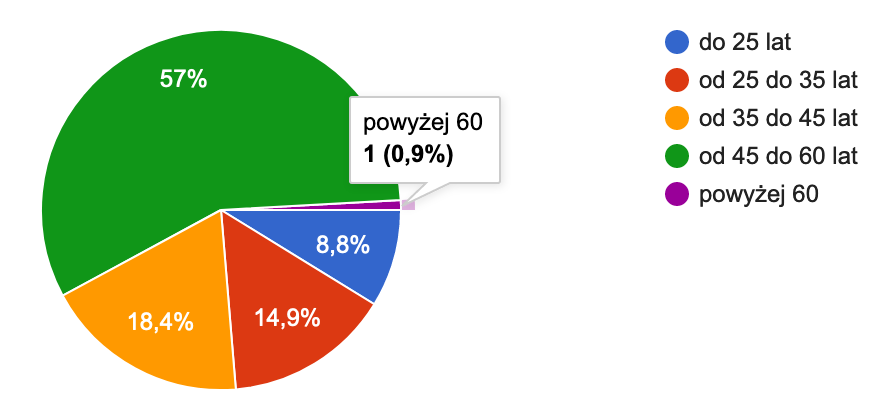
\includegraphics[width=9cm]{char_gr_bad/wiek00}
\caption{Wiek osób ankietowanych. Badania własne 2021/2022 r.}
\label{rys:wiek}
\end{figure}


% tabela wiek  - statystyka
\begin {table}[h]
\caption{Statystyki opisowe wieku grupy badanej}
\centering
\begin{tabular}{|l|c|c|}
\hline
Statystyka & Symbol & Wartość\\
\hline
Test Shapiro-Wilk & $p$ & <0,001\\
\hline
liczność danych & $n$ & 114\\
\hline
Średnia & $\bar{x}$ & 43.9\\
\hline
Odchylenie standardowe & $S$ & 10.7\\
\hline

\end{tabular}
\label{tab:wiek}
\end{table}


\subsection*{Płeć}

Badaną grupę przedstawioną  na rysunku \ref{rys:plec} stanowi  93,9\%  (108 kobiet) i  6,1\%  (7 mężczyzn). Widoczna dysproporcja jest typowa dla rozkładu płci osób zatrudnionych jako pielęgniarki/arze.

% ilustracja płeć
\begin{figure}[h]
\centering
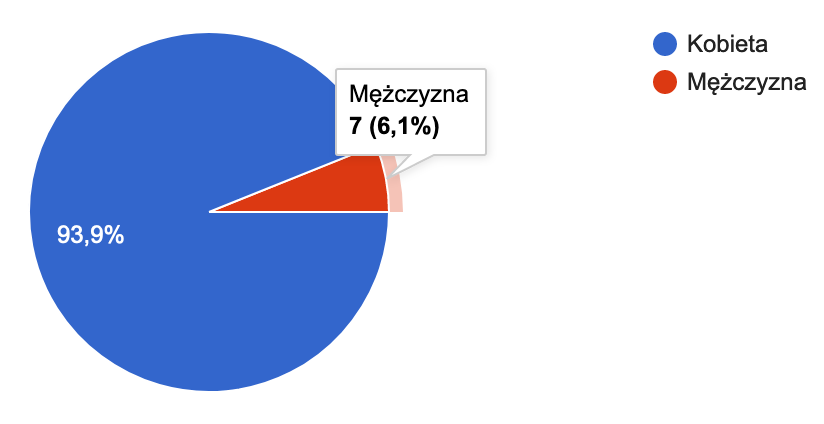
\includegraphics[width=8cm]{char_gr_bad/plec00}
\caption{Płeć osób ankietowanych. Badania własne 2021/2022 r.}
\label{rys:plec}
\end{figure}


\subsection*{Wykształcenie}


Wśród ankietowanych najliczniejszą grupę reprezentowało 57,4\%) (66 osób) z wykształceniem wyższym - Licencjat Pielęgniarstwa oraz  23,5\%  (27 osób) z tytułem Magistra Pielęgniarstwa. Niektóre osoby zaznaczyły również opcję Liceum Medyczne i  Studium Medyczne. Graficzną reprezentację rozkładu wykształcenia przedstawia rys. \ref{rys:wykszt}. Dodatkowo, rys. \ref{rys:podyplom} ilustruje kształcenie podyplomowe, podejmowane przez badaną grupę.


% ilustracja wykształcenie
\begin{figure}[h]
\centering
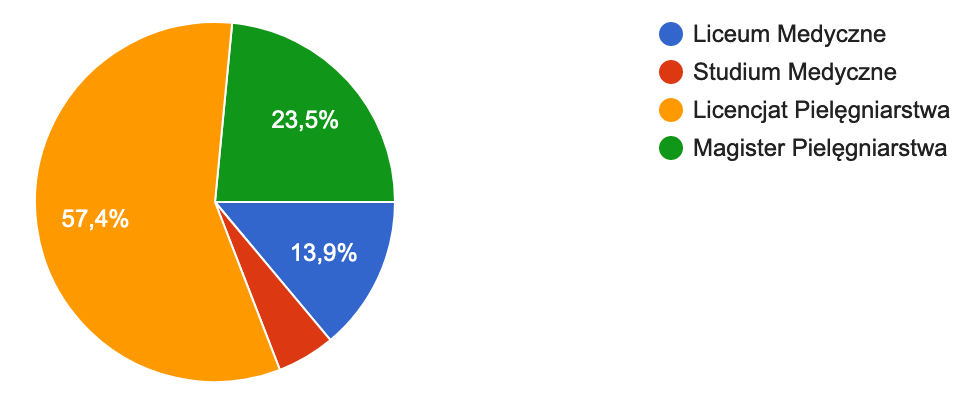
\includegraphics[width=9cm]{char_gr_bad/wyksztalc00}
\caption{Wykształcenie osób ankietowanych. Badania własne 2021/2022 r.}
\label{rys:wykszt}
\end{figure}

\begin{figure}[h]
\centering
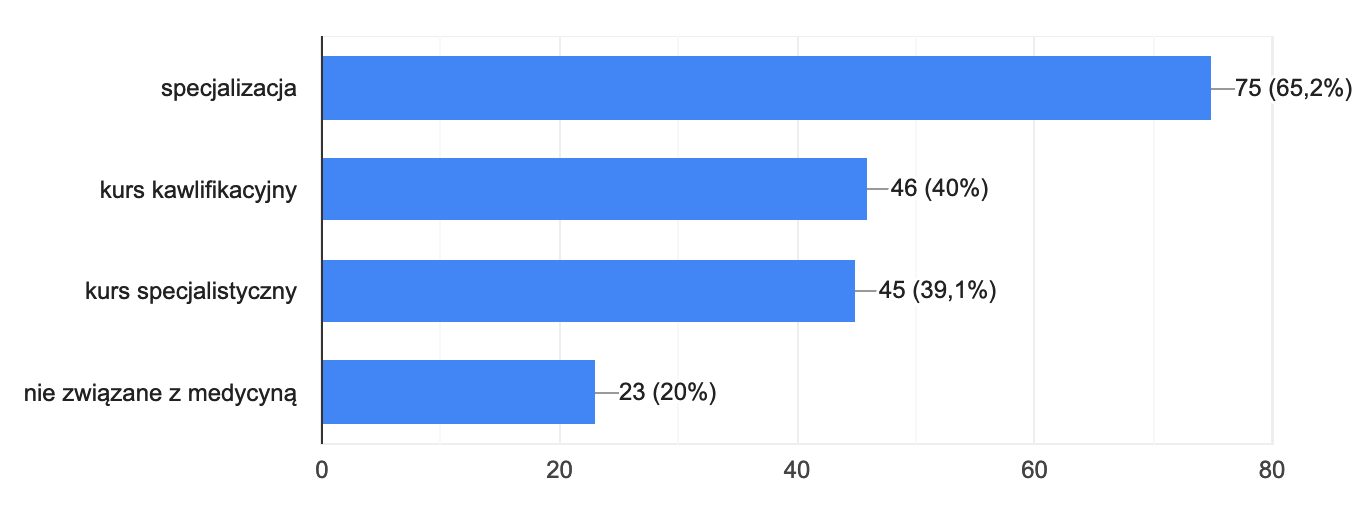
\includegraphics[width=11cm]{char_gr_bad/podyplom00}
\caption{Wykszałcenie podyplomowe osób ankietowanych. Badania własne 2021/2022}
\label{rys:podyplom}
\end{figure}


\subsection*{Stan cywilny}
Zdecydowana większość ankietowanych pozostaje  w związku małżeńskim 67,8\%  (78 osób) , w związku nieformalnym 17,4\% (20 osób). 15 \% to osoby nie żyjące w związku, w tym  8,7\%) (10 osób) rozwiedzione,  5,2\%) ( 6 osób) samotne i 0,9\%)  (1 osoba)  to wdowa. Rozkład ankietowanych pod względem stanu cywilnego ilustruje rys. \ref{rys:cywil}.

% stan cywilny
\begin{figure}[h]
\centering
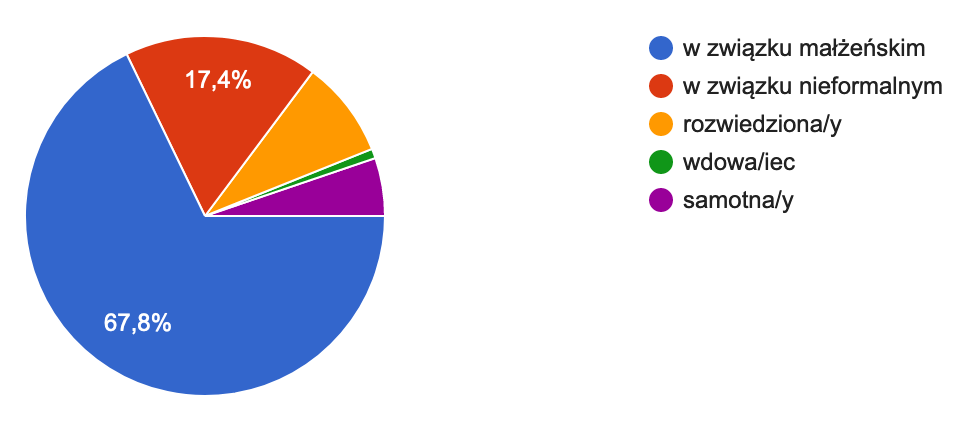
\includegraphics[width=9cm]{char_gr_bad/cyw00}
\caption{Stan cywilny ankietowanych. Badania własne 2021/2022 r.}
\label{rys:cywil}
\end{figure}

\subsection*{Miejszce zamieszkania}
Rozkład ankietowanych pod względem miejsca zamieszkania przedstawiono na rys. \ref{rys:zamiesz}. Rozkład ten okazał się być dość równomierny. Niewiele powyżej średniej stanowiła grupa 25,2\%   (29 osób) zamieszkująca  wsie. Miasta do 50 tys. mieszkańców reprezentowała grupa  20\%  (23 osoby). Tak samo liczna grupa zamieszkiwała w miastach od 50 do 150 tys. Nieco mniejsza grupa  18,3\% (21 osób) pochodziła z miast powyżej 150 tys, natomiast z miast powyżej 500 tys.  16,5\% (19 osób).
% miejsce zamieszkania
\begin{figure}[h]
\centering
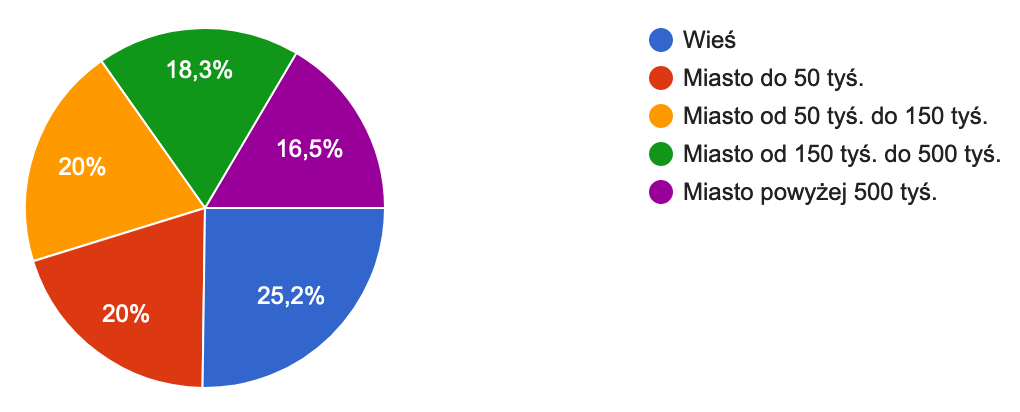
\includegraphics[width=9cm]{char_gr_bad/zamieszka00}
\caption{Miejsce zamieszkania ankietowanych. Badania własne 2021/2022 r.}
\label{rys:zamiesz}
\end{figure}

%-----------------
% Analizy statystyczne
%-----------------
\section{Opis metod analizy statystycznej}

Analizy wykonano w programie GNU PSPP, wer.: 1.4.1, oraz w programie Microsoft Excel, wer 16.60. Konwersję wyników ankiety Google do postaci tabelarycznej wykonano przy pomocy autorskiego skryptu wykonanego w programie PyCharm, wer.: 2022.1.1.

\vspace{\baselineskip} 

Wyniki testów statystycznych podano w standardzie APA \cite{apa}:\newline

\begin{equation}
    \chi^2 (lss, n) = x, p=y
\end{equation}

\vspace{\baselineskip} 
gdzie:\newline
$lss$ -liczba stopni swobody\newline
$n$ - liczność zbioru danych\newline
$x$ - obliczona wartość testu $\chi^2$\newline
$y$ - wartość prawdopodobieństwa $p$\newline


Metody statystyczne, którymi się posłużono, to:
\begin{itemize}
     \item Test Shapiro – Wilka, służy do testowania podobieństwa rozkładu danej zmiennej do rozkładu normalnego. Za pomocą tego testu, sprawdzamy czy interesujące nas zmienne mają rozkłady zbliżone do rozkładu normalnego. Test Shapiro-Wilka testuje hipotezę zerową mówiącą, że rozkład naszej zmiennej jest zbliżony do normalnego. Z tego wynika, że istotny wynik testu Shapiro-Wilka świadczy o tym, że rozkład zmiennej obserwowanej nie jest podobny do rozkładu normalnego \cite{ShapWilk}. 
    
     \item Test Pearsona $\chi^2$, to test nieparametryczny, służący do oceny zależności pomiędzy rozkładem częstości odpowiedzi w zakresie jednej zmiennej, w odniesieniu do drugiej zmiennej.
     
     \item Test Manna – Whinteya opiera się na medianach. Pozwala zweryfikować czy między porównywanymi grupami występują istotne statystyczne różnice. Stosowany jest do porównań pomiędzy dwoma grupami. Stosowany jest w przypadku rozkładów o charakterze różnym od normalnego.
    
     \item Test Kruskala – Wallisa test nieparametryczny, opierający się na medianach. Pozwala zweryfikować czy między porównywanymi grupami występują istotne statystyczne różnice. Stosowany jest do porównań pomiędzy więcej niż dwoma grupami. Stosowany jest, gdy w jednej grupie rozkład ma charakter różny od normalnego.
     
\end{itemize}



\chapter{Wyniki badań}


%-------------------------
% badania - hipotezy
%-------------------------
\section*{Badania właściwe dla stawianych hipotez}


\subsection* {Hipoteza 1 - Własne zdrowie, nie jest priorytetem  dla pielęgniarek pracujących w ponadnormatywnym czasie pracy.}



Do poparcia tezy wykorzystano odpowiedzi ankietowanych na pytanie 30 dotyczące pracy zawodowej   mimo wystąpienia choroby własnej, lub członka rodziny.
Rozkład odpowiedzi zbadano testem normalności rozkładu Shapiro - Wilka
i uzyskano wynik:  $p < 0,001$
Odpowiedzi na to pytanie przedstawia tabela \ref{tab:praca_choroba}.


% tabela wiek  - statystyka
\begin {table}[h]
\caption{Praca pomimo wystąpienia choroby}
\begin{tabular}{|c|c|c|}
\hline
odpowiedź & liczność & procent\\
\hline
zdecydowanie nie & 3 & 2,6\%\\
\hline
raczej nie & 17 & 14,8 \% \\
\hline
nie mam zdania & 3 & 2,6\%\\
\hline
raczej tak & 57 & 49,6\%\\
\hline
zdecydowanie tak & 35 & 30,4 \%\\
\hline

\end{tabular}
\label{tab:praca_choroba}
\end{table}

Uwzględniono również odpowiedzi ankietowanych na pytanie 31 dotyczące  wykorzystania zwolnienia L4, gdy są do tego wskazania.
Rozkład odpowiedzi zbadano testem normalności rozkładu Shapiro - Wilka
i uzyskano wynik:  $p < 0,001$
Odpowiedzi na to pytanie przedstawia tabela \ref{tab:L4}.

% tabela wiek  - statystyka
\begin {table}[h]
\caption{Praca pomimo wystąpienia choroby}
\begin{tabular}{|c|c|c|}
\hline
odpowiedź & liczność & procent\\
\hline
zdecydowanie nie & 11 & 9,6\%\\
\hline
raczej nie & 34 & 29,6 \% \\
\hline
nie mam zdania & 6 & 5,2\%\\
\hline
raczej tak & 46 & 40\%\\
\hline
zdecydowanie tak & 18 & 15,7\\
\hline

\end{tabular}
\label{tab:L4}
\end{table}


Analizie poddano dwie zmienne: odpowiedź ankietowanych na pytanie 3, dotyczące ilości godzin pracy miesięcznie, oraz odpowiedź na pytanie 13 czy, w celu radzenia sobie ze stresem związanym z pracą zawodową, sięga Pan/i po używki? Pierwsza zmienna ma charakter ilościowy a druga jakościowy. W celu określenia istotności statystycznej zastosowano test $\chi^2$ Pearsona. 

Istnieje korelacja pomiędzy ilością ponadnormatywnych godzin pracy a sięganiem po używki ($\chi^2 (2, 115) = 6,1152, p=0,047$)
   
\vspace{\baselineskip} 
\TODO
\newline
powyższe  i kolejne  "analizie poddano ..." zamienić stylistycznie na cos takiego: \newline
"Test statystyczny wykazał istotne statystycznie różnice globalnego poczucia koherencji (SOC) w zależności od wykształcenia (wartość statystyki testowej Kruskala-Wallisa 9,04; p=0,029). Testy post hoc pokazały, że globalne poczucie koherencji jest istotnie mniejsze u osób, które ukończyły średnią szkołę medyczną w porównaniu do absolwentów magisterskich studiów pielęgniarskich (p=0,026) – Rycina 7." \newline
lub gdy p>0,05
\newline
Test statystyczny nie wykazał istotnych statystycznie różnic poczucia zrozumiałości (PZR) w zależności od wykształcenia (wartość statystyki testowej Kruskala-Wallisa 5,37; p=0,147).

   
   

\subsection*{Hipoteza 2 - Pielęgniarki/arze mają wsparcie w godzeniu życia zawodowego i rodzinnego.}

Ankietowani  w pytaniu 26 udzielali odpowiedzi na temat wsparcia rodziny w godzeniu obowiązków domowych, oraz  pytanie 24 czy czynnie uczestniczy pan/i w życiu rodzinnym i imprezach okolicznościowych.

korelacja z
zadowolona (z perspektywy czasu)
czy wspierałaby pani decyzje dziecka
    

\vspace{\baselineskip} 
  



\vspace{\baselineskip} 
    
Zbadano zależność  występowanie konfliktów praca-rodzina od ilości godzin pracy miesięcznie.
W celu określenia istotności statystycznej zastosowano test $\chi^2$ Pearsona.  
Wynik istotności statystycznej < 0,05 pozwala konkludować że istnieje korelacja pomiędzy ilością ponadnormatywnych godzin pracy a nasileniem konfliktów na linii praca-rodzina ($\chi^2 (2, 115) = 6.423, p=0,0403$).
Test wykonano na zagregowanych danych przedstawinych w tabeli kontyngencji \ref{tab:konflikt-godziny}

% tabela kontyngencji konflikt-godziny
\begin {table}[h]
\caption{Występowania konfliktów praca-rodzina vs. ilość godzin pracy}
\begin{tabular}{|c|c|c|c|}
\hline
\multirow{2}{1cm}{konflikt} & 
   \multicolumn{3}{|c|}{liczba godzin pracy w mies.}\\
   \cline{2-4}
    &  do 169 & od 170 do 239 & 240 i więcej \\
\hline
występuje & 9 & 10 & 4 \\
\hline
nie występuje & 56 & 32 & 4\\
\hline

\end{tabular}
\label{tab:konflikt-godziny}
\end{table}
  
\vspace{\baselineskip}   

\subsection*{Hipoteza 3 - Poziom wykształcenia kadry pielęgniarskiej ma istotne znaczenie, dla  redukowania skutków traumatyzacji, wynikających z trudnych sytuacji w pracy.}


Analizie poddano dwie zmienne: odpowiedź ankietowanych na pytanie dotyczące wykształcenia, oraz odpowiedź na pytanie 12 Czy potrafi Pan/i, niwelować w.w objawy, za pomocą technik psychologicznych?. Przyjęto że obie zmienne mają charakter jakościowy. W celu określenia istotności statystycznej zastosowano test $\chi^2$ Pearsona.

Istnieje korelacja pomiędzy poziomem wykształcenia a umiejętnościami niwelowania skutków traumatyzacji ($\chi^2 (3, 115) = 7,934, p=0,0474$)

\TODO zastanowic sie nad wyrzuceniem lub przeniesieniem do innej Hip
Analizie korelacyjnej poddano dwie zmienne: odpowiedź ankietowanych na pytanie 3, dotyczące ilości godzin pracy miesięcznie, oraz odpowiedź na pytanie 10 „Czy przynosi Pan/i ,,pracę" do domu, w postaci emocji i myśli?”. Pierwsza zmienna ma charakter ilościowy a druga jakościowy. W celu określenia istotności statystycznej zastosowano test $\chi^2$ Pearsona.

    Ilość godzin pracy nie ma istotnego wpływu na przynoszenie do domu pracy w postaci myśli i emocji ($\chi^2 (2, 115) = 0,224, p=0,894$)
    
    \TODO potrzeba wsparcia  vs wyksztalcenie
    
    \TODO zamienic na traumatyzacja vs. wyksztalcenie
    
    Analizie poddano dwie zmienne: odpowiedź ankietowanych na pytanie 3, dotyczące ilości godzin pracy miesięcznie, oraz odpowiedź na pytanie 11 czy doświadcza Pan/i, zjawiska określanego jako traumatyzacja wtórna (odczuwanie, objawów psychicznych - smutek, żal, poczucie bezradności, stres) oraz objawów somatycznych, po wystąpieniu trudnej, dramatycznej sytuacji w pracy, powyżej 30 dni?”. Pierwsza zmienna ma charakter ilościowy a druga jakościowy. W celu określenia istotności statystycznej zastosowano test $\chi^2$ Pearsona. 
 
Ilość godzin pracy nie ma istotnego wpływu na odczuwanie traumatyzacji wtórnej ($\chi^2 (2, 115) = 0,8926, p=0,64$)
\vspace{\baselineskip} 

\subsection*{Hipoteza 4 - Satysfakcja zawodowa pielęgniarek i pielęgniarzy, wynika z kultury organizacji oraz nabywania kolejnych uprawnień.}
pyt 20 o satysfakcję
Analizie poddano dwie zmienne: odpowiedź ankietowanych na pytanie 7: "dotyczące wspierającego środowiska pracy oraz odpowiedź na pytanie 5, na temat zadowolenia z wyboru drogi życiowej. Obie zmienne mają charakter jakościowy. W celu określenia istotności statystycznej zastosowano test $\chi^2$ Pearsona.

Wynik testu pokazuje że istnieje korelacja pomiędzy wspierającym środowiskiem pracy a zadowoleniem pracownika z wyboru drogi zawodowej. ($\chi^2 (4, 115) = 9,53169, p=0,0491$)

\vspace{\baselineskip}

Analizie poddano dwie zmienne: odpowiedź ankietowanych na pytanie 8, o występowaniu mobbingu i hejtu w środowisku pracy, oraz odpowiedź na pytanie 5, na temat zadowolenia z wyboru drogi zawodowej. Obie zmienne mają charakter jakościowy. W celu określenia istotności statystycznej zastosowano test $\chi^2$ Pearsona.

Wynik testu pokazuje że istnieje korelacja pomiędzy toksycznym środowiskiem pracy a brakiem zadowolenia pracownika z wyboru drogi zawodowej. ($\chi^2 (4, 115) = 10,87545, p=0,028$)

\vspace{\baselineskip}
Analizie poddano dwie zmienne: odpowiedź ankietowanych na pytanie 9 na temat systemów motywacyjnych w zakładzie pracy, oraz  ponownie odpowiedź na pytanie 5. Obie zmienne mają charakter jakościowy. W celu określenia istotności statystycznej zastosowano test $\chi^2$ Pearsona.

Wynik testu nie pozwala na określenie korelacji pomiędzy stosowaniem systemów motywacyjnych a zadowoleniem pracownika z wyboru drogi zawodowej, ponieważ wartość istotności statystycznej $p$ przekracza założony próg 0,05. ($\chi^2 (4, 115) = 10,87545, p=0,272$)

\vspace{\baselineskip} 

\subsection*{Hipoteza 5 - System Opieki Zdrowotnej nie spełnia oczekiwań, w zakresie promocji, przyszłości i autonomii pielęgniarstwa.}

\vspace{\baselineskip} 

TODO: badania do hipotezy 5
czy czuje się pani bezpiecznie w pracy z koronarowirusem pytanie 18, dylemat wynikający z podnoszenia kwalifikacji, prasja społeczna wobec sytemu ochrony zdrowia 15, poparcie dla działań typu strajki pytanie 19, czy kompetencje są właściwie wykorzystane pytanie 21



pyt 15 dylemat podnosz kwal vs. pyt 21 kompetencje
\vspace{\baselineskip} 


%-----------------
% Wnioski 
%-----------------
\chapter{Wnioski}


%-----------------
% Dyskusja
%-----------------
\section{Dyskusja}
,,Dyskusja jest częścią krytyki metodologicznej i stanowi swoistą metametodę, leżącą u podstaw współczesnego myślenia naukowego, jak i stały element metod, w ramach których można ją sensownie realizować"\cite{krytyka}.


Celem badania własnego było określenie wpływu pracy zawodowej na życie osobiste pielęgniarek i pielęgniarzy czynnych zawodowo. To zagadnienie było obiektem zainteresowań badaczy różnych specjalności. Zarówno socjologów, psychologów jak i zarządzania w systemie ochrony zdrowia.  Dzięki temu, możliwe jest szerokie spojrzenie na życie, specyficznej grupy zawodowej jaką są pielęgniarki. Możliwe jest zaobserwowanie pewnych zjawisk, np. wypalenia zawodowego, określenie przyczyn ich występowania, a następnie wdrożenie działań profilaktycznych, naprawczych czy protekcyjnych. Wyniki kolejnych badań wzbogacają wiedzę, służą rozwojowi pielęgniarstwa. Ze względu, iż temat jest rozległy i obejmuje wiele dziedzin życia społecznego, badacze nadal poszukują odpowiedzi na pytania : czy wykonując tak odpowiedzialny i wyczerpujący zawód, można prowadzić szczęśliwe życie osobiste? Czy empatia pomaga, czy przeszkadza w wykonywaniu tego zawodu? Jakie niebezpieczeństwa niesie wykonywanie tego zawodu? Niniejsza praca również podejmuje próbę odpowiedzi na te pytania.

%-------------
% hipoteza 1
%-------------
\subsection*{hipoteza 1:} 
Poziom świadomości pielęgniarek i pielęgniarzy na temat zagrożeń, wynikających z pracy w ponadnormatywnym czasie pracy, powinien mieć istotne znaczenie na decyzję o podjęciu dodatkowej działalności zawodowej. 

Jak wykazano w części teoretycznej, praca zawodowa pielęgniarek i pielęgniarzy, zwłaszcza praca w godzinach nocnych i ponadnormatywnym wymiarze pracy niesie niekorzystne skutki dla stanu biopsychospołecznego człowieka. Świadomość tego faktu jest niewystarczająca, lub schodzi na plan dalszy, wobec różnych potrzeb, które podlegają zmianom w trakcie życia. Tu musi być wynik istotności statystycznej

W czerwcu 2021 r Stowarzyszenie Pielęgniarki Cyfrowe przeprowadziło badanie sondażowe, w którym wzięło udział 2459 osób. 91,9\% to pielęgniarki i pielęgniarze. 8,1\% to położne/i.  94,3\%   osób ankietowanych w podstawowym miejscu pracy zatrudnionych jest w pełnym wymiarze etatu. Pozostali wykonują zawód na podstawie innych form zatrudnienia. 45,4\%  pracuje dodatkowo: kontrakty, umowy zlecenia, a nawet cały etat. Osoby zatrudnione w ramach umowy o pracę deklarowały powyżej 200 godzin pracy w miesiącu. Zdecydowana większość respondentów podawała iż powodem dodatkowej pracy są względy ekonomiczne, plany życiowe - 25,7\%,  podstawowa egzystencja -  23,1\%, 9,5\%. godzi się na dodatkowe dyżury z powodu braków kadrowych. Pojawiły się również powody takie jak samotność, pracoholizm, chęć samorealizacji \cite{cyfrowe}. W badaniach własnych, w których wzięło udział 115 studentów i absolwentów Wyższej Szkoły Medycznej  w Legnicy na kierunku pielęgniarstwo drugiego stopnia, wyniki  przedstawiają się następująco: 65,2\% (75 osób) pracuje w jednym miejscu pracy, 27,8\%  (32 osoby) w dwóch, a 7\%  (8 osób) w więcej niż dwóch.  Ze 115 osób 14 osób pracuje powyżej 200 godzin miesięcznie, co stanowi, 12,2\% ankietowanych. 8 osób deklaruje pracę powyżej  240 godzin miesięcznie.


Nie bez znaczenia jest fakt, że zagrożenia  dla zdrowia, wynikające z pracy w ponadnormatywnym wymiarze mogą ulec intensyfikacji czy zniwelowaniu, poprzez kulturę organizacji. Wśród ankietowanym studentów Wyższej Szkoły Medycznej w Legnicy 34,8\% (40 osób) uważa, że środowisko miejsca pracy jest toksyczne, występuje mobbibg i hejt. 36,5\% (42 osoby) podaje, że w miejscu ich pracy takie zjawiska nie występują. Pozostałe osoby są niezdecydowane w tej kwestii.  Podobne wyniki obserwuje się w pracach innych badaczy. Na uwagę zasługują wnioski z badania ,,mobbing w środowisku pracy pielęgniarek" przeprowadzonego za pomocą sondażu diagnostycznego wśród pielęgniarek województwa świętokrzyskiego w 2010 roku. Gdzie zaobserwowano działania dyskryminacyjne i o charakterze mobbingowym wobec personelu podnoszącego swoje kwalifikacje i wykształcenie. W badaniu tym dokonano porównań z podobnymi w województwie śląskim, mazowieckim i zachodniopomorskim \cite{mobbing}. Z kolei Żuchowski w badaniach, przeprowadzonych na terenie województwa mazowieckiego i podlaskiego, w którym wzięło udział 140 respondentów, wykazuje, że zjawisko mobbingu kadry zarządzającej pielęgniarkami, w stosunku do podwładnych to liczba, rzędu 27,8\% \cite{zuchowski}. Z danych Ogólnopolskiego Klubu Antymobbingowgo wynika, iż liczba pracowników Ochrony Zdrowia jest niedoszacowana i na pewno wyższa\cite{grabowski}, mimo, iż termin mobbing wprowadzono do znowelizowanego Kodeksu Pracy w 2004 roku \cite{kodeks}.


Wykonywanie obowiązków zawodowych w trakcie aktywnej choroby własnej, czy bliskiego, świadczy o prawdziwości założonej hipotezy. 49,6\% (57 osób) badanych zaznacza, że raczej pracuje mimo wystąpienia choroby własnej czy członka własnej rodziny. 30,4\% (35 osób) zdecydowanie wykonuje swoje obowiązki zawodowe w tym czasie. 68,8\% (45 osób) nie korzysta ze zwolnienia lekarskiego, gdy są do tego wskazania. Jest to wysoce niepokojące zjawisko, gdyż aby wykonywać swoje zadania w pracy zawodowej, muszą one stosować leki, które np. zniwelują objawy przeziębienia czy grypy. Abstrahując od etycznego wymiaru takich działań,  ich konsekwencji dla pacjenta, placówki, to niosą one konkretne skutki dla zdrowia pielęgniarki. Metha i współpracownicy opublikowali w marcu 2022 wyniki ogólnokrajowego prospektywnego, kohortowego badania  w USA. Czternaście tysięcy pięćset czterdzieści dwie  pielęgniarki w wieku 25-42 lata uczestniczyło w badaniu Nurses Health Study II. W przedziale czasowym 1989 - 2018,  co dwa lata monitorowano stosowanie przez nie antybiotyków i jednocześnie przeprowadzano testy poznawcze. Wyniki porównywano z danymi osób, które przyjmowały antybiotyków niewiele lub wcale. Wyniki były niepodważalne: Pielęgniarki, które często, czy długotrwale stosowały antybiotyki uzyskały zdecydowanie niższe parametry uczenia się, pamięci roboczej, szybkości motorycznej czy utrzymania uwagi. Sytuację taką autorzy opisują przyśpieszonym starzeniem mózgu, nawet o 3-4 lata.  Co dla  pielęgniarki polskiej o średniej wieku - 53 lata, powinno mieć znaczenie \cite{statystyka}.  Naukowcy  wiążą zaburzenia poznawcze z  kondycją mikrobiomu jelitowego \cite{metha}.
Dane o chorobach przewlekłych i współistniejących badanej grupy  studentów WSM w Legnicy  również  świadczą o prawidłowym założeniu hipotezy, gdyż aż 45,2\% (52 osoby) choruje na choroby przewlekłe, a 5,2\% (6 osób) na choroby współistniejące.


24,4\% (28 osób) ankietowanych uważa, że jest wypalona zawodowo, a 13,9\% (16 osób) respondentów nie ma zdania na ten temat. Jak wiadomo, wypalenie zawodowe jest ogromnym problemem pracowników ochrony zdrowia, jednocześnie, ta grupa zawodowa jest na nie najbardziej narażona,  z pośród pracowników innych profesji \cite{wypal}. Rezmerska i współautorki, w badaniach na temat specyfiki pracy, a wypalenia zawodowego w opinii pielęgniarek,  przekonują, iż poziom wypalenia zawodowego, jest zróżnicowany w zależności od specyfiki oddziału. Jest on wyższy, w oddziałach zabiegowych, u pielęgniarek pracujących w systemie zmianowym \cite{zmiany}. Natomiast Breisert w badaniach przeprowadzonych w Poznaniu na grupie 138 pielęgniarek pokazuje, że najwięcej osób wypalonych zawodowo jest zatrudnionych na pediatrii, onkologii i psychiatrii, natomiast zadecydowanie mniej na internie. Wymagania dotyczące specyficznego kontaktu z chorym dzieckiem, czy chorym z nowotworem, nieustanne stykanie się z cierpieniem, nieustanny, przewlekły stres oraz brak poczucia sensu własnej działalności, obciążenie pracą, brak systemów motywacyjnych, nieodpowiednie zarobki składają się na stale zwiększającą się liczbę osób wypalonych zawodowo \cite{breisert}.


%-------------
% hipoteza 2
%-------------

\subsection*{hipoteza 2:} 

Czy  pielęgniarki/arze mają wsparcie w godzeniu życia zawodowego i rodzinnego? 
 43,4\%  (50 osób) ankietowanych badania własnego spędza w pracy od 170 do 260 godzin, co przekłada się np. przy 170 godzinach na około:  7 dyżurów dobowych, 14 dyżurów dwunastogodzinnych. Przy 260 godzinach te liczby to: około  10 dyżurów dobowych,  20 dyżurów dwunastogodzinnych. Rekordzistki w trakcie indywidualnych rozmów przyznają się do 72 godzin nieprzerwanej pracy, bądź 2 dni wolnych w miesiącu \cite{cyfrowe}.  Wykładnia prawa, wyraźnie mówi, że zasadnicze normy czasu pracy obowiązujące pracowników podmiotów leczniczych wynoszą na dobę 7 godzin i 35 minut na dobę, oraz 37 godzin i 55 minut na tydzień. Jest to średnia, której nie można przekraczać w trzymiesięcznym okresie rozliczeniowym \cite{okres}. Ustawa o działalności leczniczej nie reguluje  jednak wprost limitu pracy w godzinach nadliczbowych. Pośrednio wynika to z maksymalnej normy czasu pracy w wymiarze 48 godzin tygodniowo \cite{klauzula}.
  63,5\%  (73 osoby) twierdzi, że przynosi pracę do domu w postaci myśli i emocji. 38,3\% (44 osoby) doświadcza traumatyzacji wtórnej. W badanej grupie 37,4\%  (43 osoby) potrafi niwelować objawy takie jak: smutek, żal, poczucie bezradności, przewlekły stres. 33,9\%  (39 osób) nie potrafi stosować technik psychologicznych do poradzenia sobie z sytuacją trudną, a 28,7\%  (33 osoby) nie opowiedziało się jednoznacznie za lub przeciw. 13,9\% (16 osób) w celu rozładowania stresu sięga po używki. 47\% (54 osoby) odczuwa dylemat wewnętrzny, wynikający z konieczności ciągłego podnoszenia kwalifikacji, co wiąże się z ograniczeniami w życiu osobistym. Przy tak kategorycznych danych 80\% (92 osoby) ankietowanych stwierdza, że w ich życiu nie występuje konflikt na linii praca - rodzina i odwrotnie. 73 (84 osoby) uważa, że praca nie jest powodem niezgody z życiowym partnerem, 77,4\%  (89 osób) twierdzi, że są wspierane w godzeniu obowiązków domowych z pracą. 73,9\% (85 osób) ma czas dla rodziny i czynnie uczestniczy w życiu rodzinnym i imprezach okolicznościowych. Tylko 16,5\% (19 osób) kiedykolwiek rozważało rezygnację z zawodu, na rzecz szczęścia rodziny. Równie spektakularnym wynikiem jest odpowiedź na pytanie o pasję pozazawodową. Aż 72,2\% (83 osoby) podało, iż rozwija pasję pozazawodową.  W badaniach  przeprowadzonych w Centrum Onkologii w Bydgoszczy, w 2011 roku, na grupie 72 pielęgniarek i pielęgniarzy, dotyczące analizy jakości życia pracowników ochrony zdrowia, Kurowska i Klatt  wykazują, że w badanej grupie wystąpił wysoki poziom wsparcia ze strony partnera życiowego. Także ogólne wsparcie rodziny, było na poziomie wysokim, przy czym najwyżej oceniono wsparcie emocjonalne \cite{poziom}. Natomiast w 2017 roku zespół badaczy Polskiego Pomiaru Postaw i Wartości przeprowadził badanie, w którym wzięło udział 1627 osób z zawodowej grupy pielęgniarskiej. Zdecydowanie większa liczba osób deklarowała, że udaje się jej zachować równowagę między działalnością zawodową i rodzinną - 30,6\% było zdecydowanych w tej kwestii, a 42,1\% podało odpowiedź, że taką równowagę raczej zachowuje. Tylko 28\% badanych osób, byłoby skłonnych zrezygnować z pracy, dla dobra rodziny. W tym badaniu  56,7\% neguje wpływ pracy na życie rodzinne i twierdzi, że potrafi zachować dystans między pracą, a czasem z rodziną, ale 37\% nie posiada takiej umiejętności. \cite{komunikat}.
Podsumowując dyskusję na ten temat, należy wyrazić uznanie dla osób wybierający zawód wymagający ciągłego doskonalenia i niosący ogrom poświęceń w życiu osobistym, jednocześnie realizując obie role.



%-------------
% hipoteza 3
%-------------
\subsection*{hipoteza 3:} 

Zawodowa grupa pielęgniarska, kształci się, aby niwelować skutki traumatyzacji, wynikające z trudnych sytuacji w pracy. Traumatyzacja wtórna określana do niedawna jako zmęczenie współczuciem, przypisywanym pielęgniarkom, a następnie innym zawodom pomocowym, spowodowała przeniesienie traumy z ofiary na terapeutę \cite{figley}. Na traumatyzacje narażone są osoby o wysokim stopniu inteligencji emocjonalnej. Zwłaszcza jej składowej empatii. Natomiast Wilczek - Rużyczka twierdzi na podstawie wieloletnich badań własnych i analizy wyników badań innych badaczy, że empatia pełni rolę ochronną, a ,,wysoki poziom empatii, jest nie tylko wartością psychologiczną, terapeutyczną, lecz również powinnością moralną i staje się kryterium profesjonalizmu."  Pielęgniarka wchodząc w relację z pacjentem, odczuwa bliskość, która zaspokaja często potrzeby obu stron, jednocześnie nie traci własnej tożsamości \cite{wilczek}. Wśród osób, które wzięły udział w badaniu  15,7\% (18 osób) odpowiedziało, że empatia była głównym kryterium wyboru przez nie zawodu, a 22,6\% (26 osób) przychylało się do tej odpowiedzi. Trening empatii oraz kształcenie się w  rozpoznawaniu, niwelowaniu niekorzystnych skutków traumatyzacji,  ma ogromne znaczenie dla życia osobistego pielęgniarki. Biorący udział w badaniu własnym,  posiadają wykształcenie wyższe - 57,4\% (66 osób) licencjat pielęgniarstwa,  23,5\% (27 osób)to magister pielęgniarstwa. Znamienita większość zdała egzamin specjalizacyjny - 65,2\% (72 osoby). Ankietowani wykazują posiadanie uprawnień zawodowych potwierdzonych zaświadczeniami, certyfikatami i dyplomami, również niezwiązanymi z zawodem wykonywanym, także magistra innego kierunku. Wśród wielu czynników ryzyka wtórnej traumatyzacji wymienia się poziom wykształcenia. Wyższe wykształcenie oraz poczucie satysfakcji z pracy pełni rolę ochronną, natomiast osoby o niższym stopniu wykształcenia są bardziej podatne, na zmęczenie współczuciem \cite{oginska}.



29,6\% (34 osoby) badanych zdecydowanie czuje presję społeczną, wynikająca z oczekiwań wobec systemu ochrony zdrowia. 35,7\% (42 osoby) zaznaczyło odpowiedź ,,raczej tak". Ponadto 11,3\% (13 osób)  czuje dylemat wewnętrzny, a 35,7\%  (41 osób) przyznaje, że raczej czuje, dylemat związany z koniecznością ciągłego podnoszenia kwalifikacji. W przytaczanym wcześniej komunikacie z badań na temat życia rodzinnego i zawodowego. 79,9\% uznało, że zawód wymaga od nich nieustannego podnoszenia kwalifikacji zawodowych \cite{komunikat}. W badaniu własnym 46\% (53 osoby) ankietowanych doświadczyło przemocy słownej lub fizycznej ze strony pacjenta, a 33\% (38 osób) uznało, że, ,,raczej tak".  Grudzień i współpracownicy w pracy oryginalnej - opinie personelu medycznego na temat agresywnych zachowań pacjentów przedstawiają wyniki badania sondażowego, w którym udział wzięło 115 przedstawicieli zawodów medycznych. Wyniki są zbliżone do badania własnego - 46,2\% to kontakt z agresją w stosunku do pielęgniarek. Jest to zarówno agresja słowna, wulgaryzmy oraz lekceważące wypowiadanie się o personelu \cite{grudzień}. 

46,1\% (53 osoby) nie  czuje się bezpiecznie w pracy w zagrożeniu koronarowirusem. Jest to niepokojący wynik, biorąc pod uwagę, że pandemia została znacznie ograniczona przez szczepienia antywirusowe. Zapewne jest to liczba zdecydowanie mniejsza, niż na początku epidemii, gdzie fundamentalne prawo pracownika, do bezpieczeństwa własnego w pracy i poza nią, utraciło moc.

 37,4\% (38 osób) potrafi niwelować objawy traumatyzacji wtórnej za pomocą technik psychologicznych, a 27\% (31 osób) zdecydowanie czuje i 20\% (23 osoby) raczej czuje potrzebę korzystania ze wsparcia psychologicznego dla pracowników medycznych. Pozostałe osoby zdecydowanie, nie potrzebują takiego wsparcia - 9,6\%  (11 osób) i 30,4\% (35 osób) raczej nie potrzebują wsparcia w tym zakresie. Ogińska-Bulik w badaniach przeprowadzonych w 2019 roku na grupie 200 przedstawicieli personelu medycznego, w tym 35\% stanowiły pielęgniarki, przedstawia wyniki wskazujące na wysokie i średnie nasilenie wtórnego stresu wśród pracowników po traumie. Wnioski zachęcają do ,,rozwoju umiejętności i korzystania ze wsparcia społecznego, w celu redukowania negatywnych i występowania pozytywnych konsekwencji wtórnej ekspozycji na traumę" \cite{trauma}. 

% ----------
% hipoteza 4
% ----------
\subsection*{hipoteza 4:} 
Satysfakcja zawodowa pielęgniarek i pielęgniarzy, wynika z kultury organizacji oraz nabywania kolejnych uprawnień. Hipotezę tę poddano weryfikacji osób badanych i aż, 55,6\%  (64 osoby) odczuwa satysfakcję, wynikającą z autonomii zawodu - nabywania kompetencji, uprawnień, prowadzenia badań naukowych.   85,2\% (98 osób) jest zadowolona z wyboru drogi zawodowej. 71,3\% (82 osoby) uważa z perspektywy czasu, że dokonało właściwego wyboru ścieżki zawodowej, a 56,5\% (65 osób) ankietowanych wspierałoby własne dziecko, gdyby chciało się spełniać w pielęgniarstwie. Mimo to, 36,5\% (42 osoby) podkreśla, że w zakładzie pracy, w którym pracuje,   zdecydowanie nie stosuje się systemów motywacyjnych, 40,9\% (47 osób), że raczej nie. Tylko 13,9\% (16 osób) twierdzi, że raczej istnieją takie systemy. 5,2\% (6 osób) ankietowanych uważa, że środowisko pracy jest wspierające i 48,7\%  (56 osób)  uważa, iż jest raczej wspierające. Natomiast zdecydowanie toksyczne środowisko pracy występuje u 7\% (8 osób) ankietowanych, a 27,8\%  (32 osoby) podało odpowiedź raczej tak. W badaniach  Borowskiej i współpracowników na 130 aktywnych zawodowo pielęgniarkach Uniwersyteckiego Szpitala Klinicznego w Białymstoku, 41,5\% osób określiło własną satysfakcję zawodową jako wysoką, a 63\% czuło się docenioną w pracy zawodowej. Zdaniem co trzeciej osoby, atmosfera w pracy ma kluczowe znaczenie dla poczucia satysfakcji zawodowej. Pielęgniarki - 60\%, w tym badaniu określiły  pozycję swojego zawodu, wśród innych zawodów na poziomie średnim. W pytaniu o prestiż zawodu, ankietowani - 45\% uznało kwalifikacje zawodowe, 40\% wykształcenie, 33\% samodzielność i niezależność zawodu \cite{zbiorowa}. Interesujące są również badania Skorupskiej  i Machowicz, gdzie badani w 92\% uważają, że pielęgniarka jest równorzędnym członkiem zespołu w w opiece nad pacjentem \cite{skorupska}. O ocenę poziomu satysfakcji zawodowej wśród pielęgniarek onkologicznych pokusiły się organizatorki 22 ogólnopolskiej konferencji pielęgniarek onkologicznych w Białymstoku w 2018 roku. Badaniu poddało się dobrowolnie 218 uczestniczek z ośrodków onkologicznych w kraju. Średnia wartość satysfakcji z pracy wyniosła 67,10 punktów. Uczestniczki podkreślały zadowolenie z umiejętności zawodowych swojego przełożonego, wagi własnej pracy. Co ciekawe nie wykazano zależności satysfakcji z wykształceniem, ani stażem pracy. Natomiast wyższy poziom satysfakcji prezentowały osoby w związkach małżeńskich \cite{onkologiczne}. Przekrojowy sondaż Aiken i współpracowników wśród  33 tysięcy 659 pielęgniarek w 488 szpitalach w 12 krajach europejskich wykazał niezadowolenie z pracy  w 11- 56\% badanych, 19-49\% planowała odejść z pracy \cite{termedia}. Podobne wnioski płyną z wyników badań Dallora  i współpracowników, gdzie 26\% pielęgniarek i pielęgniarzy jest bardzo, albo raczej nieusatysfakcjonowanych pracą zawodową \cite{dalora}. Wiedzę i postawy pielęgniarek na temat praktyki opartej na dowodach naukowych oceniała Gotlib i współautorzy Warszawskiego Uniwersytetu Medycznego w 2014 roku. Uczestnicy badania znali zaczenie terminu EBM w 42\%, dla 34\% to nowoczesne wykonywanie zawodu, 36\% zamierza aktualizować wiedzę zgodnie z doniesieniami naukowymi, a 41\% uważa, że są one przydatne w praktyce zawodowej \cite{gotlib} Również Młynarska w swojej pracy doktorskiej  Poszukiwanie czynników wpływających na wykorzystanie przez pielęgniarki Evidence-Based Nursing w praktyce zawodowej ocenia poziom wiedzy, postaw i umiejętności badanych 830 pielęgniarek/rzy z całej Polski  w 2018/19 roku. Wykazała, ze pielęgniarki z wykształceniem wyższym cechują się największą wiedzą i umiejętnościami związanymi z EBM, chętnie je  pogłębiają i wykorzystują. w praktyce zawodowej \cite{EBM}. Badania własne określają satysfakcję zawodową w oparciu o kulturę organizacji i kolejne stopnie wykształcenia, autonomię zawodu i możliwość prowadzenia prac badawczych. Inni badacze umieścili w kwestionariuszach pytania o wynagrodzenie, docenienie, prestiż środowiska zawodowego i uznanie wśród pacjentów. Całościowe spojrzenie na zjawisko satysfakcji zawodowej, ewaluuje wraz z postępem technologicznym, oczekiwaniami pielęgniarek i ich miejsca w systemie ochrony zdrowia. Szczególnie istotna powinna praktyka oparta na dowodach medycznych. Nowoczesne pielęgniarstwo, to prestiż wyrażony krytycznym myśleniem na każdym etapie kontaktu i pracy z pacjentem, własnych kompetencji, możliwości systemu ochrony zdrowia oraz działaniem popartym dowodami naukowymi, wiedzą ekspertów z danej dziedziny. Natomiast brak satysfakcji zawodowej skutkuje poważnymi konsekwencjami dla systemu opieki zdrowotnej jak i samej pielęgniarki.

%------------
% hipoteza 5
%------------
\subsection*{hipoteza 5:} 
System Opieki Zdrowotnej nie spełnia oczekiwań, w zakresie promocji, przyszłości i autonomii pielęgniarstwa. W poprzednich rozważaniach przedstawiono dyskusję  na temat środowiska pracy ankietowanych w zakresie wsparcia, bezpieczeństwa, systemów motywacyjnych, hejtu  i agresji. Na tych polach występuje odczuwalny deficyt. Aż 74,8\%  (86 osób) popiera działania przedstawicieli zawodu zmierzające do poprawy sytuacji pielęgniarek i położnych w Polsce.  66\% (76 osób) uważa, że kompetencje pielęgniarskie, nie są właściwie wykorzystane w Systemie Ochrony Zdrowia. Wyniki badania przeprowadzonego w Szpitalu Specjalistycznym w Jaśle w 2010 roku, w których wzięło udział 130 pracowników szpitala innych niż pielęgniarki pokazują uznanie szerokich kompetencji pielęgniarskich, traktowanie pielęgniarstwa jako sztuki, samodzielnej nauki, rolę autonomicznych interwencji pielęgniarskich, zaufanie oraz solidaryzowanie się z roszczeniami pielęgniarek \cite{skorupska}. Komunikat z badań - Opinie o protestach pielęgniarek z grudnia 2000 przedstawia bardzo wysokie - 90  poparcie  społeczne dla protestujących pielęgniarek \cite{cebos}. Natomiast w 2021 roku badanie przeprowadzone na próbie 1161 osób ukazało 49\% poparcie dla strajku medyków, i aż 53\% uważa, że oczekiwanie finansowe pielęgniarek są adekwatne, a 17\%, że zbyt małe \cite{cebos2}. W 2019 roku firma Manpover Life Science we współpracy z Polską Federacją Szpitali stworzył raport - niedobór talentów w branży medycznej. Badanie objęło 71 szpitali w całej Polsce zrzeszonych w Polskiej Federacji Szpitali. W swoim opracowaniu wykazuje zapotrzebowanie na stanowiska pielęgniarek wszystkich specjalności, przez 72\% szpitali. Podkreśla brak integralnej, przyszłościowej wizji kształcenia kadr medycznych, dostosowanej do zmieniających się okoliczności, wyzwań zdrowotnych. Naświetla zjawisko emigracji zawodowej,  do krajów dobrze przygotowanych, do wykorzystania potencjału absolwentów kierunków medycznych polskich uczelni \cite{federacja}.
Oczekiwania pielęgniarek wobec SOZ, to nie tylko oczekiwania finansowe. Badania przeprowadzone przez studentów Warszawskiego Uniwersytetu Medycznego, wśród pielęgniarek dotyczą oczekiwań personelu pielęgniarskiego w zakresie organizacji i realizacji edukacji zdrowotnej dla pacjentów.  Pielęgniarki oczekują powstania zespołów edukacyjnych. W ich skład wchodzili by profesjonaliści różnych specjalności, w tym psycholog. Edukacja powinna się rozpocząć w poradni, na długo przed rozpoczęciem procedury na oddziale. Na oddziałach oczekiwane są poradniki i programy edukacyjne \cite{soz}.
Belowska, w swojej pracy doktorskiej na temat: ,,Ocena wpływu kształcenia na odległość na wiedzę i postawy pielęgniarek wobec praktyki zawodowej opartej na dowodach naukowych", dokonuje przeglądu i analizy polskiego piśmiennictwa naukowego z dziedziny EBM, ale także opracowuje narzędzie dydaktyczne i dokonuje ewaluacji działania kursu kształcącego z obszaru EBM na odległość. W swojej rozprawie doktorskiej ocenia wiedzę pielęgniarek w tym zakresie jako niewystarczającą i zgłasza potrzebę poprawy tej sytuacji. Zaproponowana przez nią platforma e-learningowa, okazała się być skutecznym i satysfakcjonującym narzędziem, zarówno w kształceniu uniwersyteckim jak i podyplomowym \cite{belowska}.



\chapter*{Streszczenie}



\appendix



%-----------------
% Bibliografia
%-----------------
\begin{thebibliography}{99}
\addcontentsline{toc}{chapter}{Bibliografia}
\bibitem{who}{ State of Worlds Nursing 2020. Investing in education, job and  leadership; https://apps.who.int/iris/handle/10665/331677. [dostęp 05.02.2022]}
\bibitem{rap}{Najbardziej poważane zawody przez Polaków w 2021;\newline https://swresearch.pl/news/najbardziej-powazane-zawody-przez-polakow-w-2021. [dostęp 05.02.2022]}
\bibitem{zro}{Historia medycyny; https://historiamedycyny.pl/ [dostęp 05.02.2022]}
\bibitem{tlo}{Maksymowicz A. Zagadnienia zawodowe pielęgniarstwa na tle historycznym. Warszawa: Wydawnictwo Lekarskie PZWL; 1977: 6-14}
\bibitem{flo}{Bostridge M. Florence Nighitingale -The lady with lamp;\newline https://www.bbc.co.uk/history/british/victorians/nightingale-01.shtml\newline [dostęp 05.02.2022]}
\bibitem{linda}{Richards L. Reminescences of Linda Richards. Americas firsttrained nurse. Boston: Whitcomb \& Barrows; 2015}
\bibitem{rada}{Poznańska S. Pielęgniarstwo wczoraj i dziś. Warszawa: Wydawnictwo Lekarskie PZWL;1988: 13-25}
\bibitem{ikon}{Supady J. Początek nowoczesnego pielęgniarstwa w XIX wieku. Health Promotion and Physical Activity. 2019; 2(7): 1-4}
\bibitem{ikonpol}{Slosorz T. Kształcenie pielęgniarek w ujęciu historycznym. Polski Przegląd Nauk o Zdrowiu. 2014; 4(41:298-304)}
\bibitem{szkol}{Iżycka-Kowalska A. Powstanie Warszawskiej Szkoły Pielęgniarstwa i jej rozwój w latach 1921-1928. Warszawa; Wydawnictwo Lekarskie PZWL; 1989}
\bibitem{50}{Kaniewska-Iżycka J. Rozwój pielęgniarstwa polskiego do 1950 roku. Materiały pomocnicze do historii zawodu pielęgniarskiego cz.1. Centrum Metodyczne Doskonalenia Nauczycieli Średniego Szkolnictwa Medycznego; 1987}
\bibitem{czas}{Wolska-Lipiec K. Czasopisma;\newline http://www.wmpp.org.pl/pl/wydawnictwa-pielegniarskie/czasopisma.html. [dostęp 11.02.2022]}
\bibitem{spec}{Hutner R. Kuźnia koncepcji pielęgniarskich. Pielęgniarstwo 2000; 1992; 3:22}
\bibitem{model}{Ministerstwo Zdrowia. Nowe kompetencje pielęgniarek i położnych. Warszawa; Fundusze Europejskie. Wiedza Edukacja Rozwój; 2020:6}
\bibitem{deter}{Sak-Skowron M. Determinanty satysfakcji z pracy. Studium teoretyczne. Marketing i zarządzanie. 2017; 2(48):243-253}
\bibitem{usta}{Wilczewska L. Rozwój zawodu pielęgniarskiego w ujęciu historycznym. Biuletyn Naczelnej Izby Pielęgniarek i Położnych. Warszawa; 1994}
\bibitem{1935}{Gnich J. Ustawa o zawodzie z 1935 r.;\newline http://www.wmpp.org.pl/pl/ustawa-o-zawodzie.html. [dostęp 11.02.2022]}.
\bibitem{1996}{Ustawa z dnia 5 lipca 1996 r. o zawodach pielęgniarki i położnej.;\newline https://isap.sejm.gov.pl/isap.nsf/DocDetails.xsp?id=WDU19960910410\newline [dostęp 11.02.2022]}
\bibitem{2011}{Ustawa z dnia 15 lipca 2011 r. o zawodach pielęgniarki i położnej.; https://isap.sejm.gov.pl/isap.nsf/DocDetails.xsp?id=wdu20111741039\newline [dostęp 11.02.2022]}
\bibitem{nipip}{Ustawa z dnia 1 lipca 2011 r. o samorządzie pielęgniarek i położnych.; http://isap.sejm.gov.pl/isap.nsf/DocDetails.xsp?id=WDU20111741038\newline[dostęp 11.02.2022]}
\bibitem{prawo}{Karkowska D. Prawo medyczne dla pielęgniarek. Warszawa: Wolters Kluwer; 2020:48}
\bibitem{akty}{Akty prawne w dziedzinie pielęgniarstwa.; https://isap.sejm.gov.pl/isap.nsf/ ByKeyword.xsp?key=pielęgniarstwo [dostęp 11.02.2022]}
\bibitem{strategia}{ Ministerstwo Zdrowia. Polityka wieloletnia państwa na rzecz pielęgniarstwa i położnictwa w Polsce. Warszawa; Fundusze Europejskie. Wiedza Edukacja Rozwój; 2020: 1-106}
\bibitem{federic}{ Laloux F. Pracować inaczej. Nowatorski model organizacji inspirowany kolejnym etapem rozwoju ludzkiej świadomości. Warszawa; Studio Emka; 2015}
\bibitem{ile}{Strzelec P. Nowe uprawnienia, nowe roszczenia-aspekty odpowiedzialności prawnej pielęgniarek i położnych. Bydgoszcz; Okręgowa Izba Pielęgniarek i Położnych; 2018;\newline http://www.oipip.bydgoszcz.pl/public/system/files/articles/571/ 736-nowe-uprawnienia-nowe-roszczenia-prezentacja.pdf [ dostęp 11.02.2022]}
\bibitem{strajk}{Związek i jego historia. Ogólnopolski Związek Zawodowy Pielęgniarek i Położnych; https://ozzpip.pl/about/ [dostęp 11.02.2022]}.
\bibitem{julia}{Osiecka J. Powrót do młodych lat;\newline https://www.queensilvianursingaward.com/pl-stories/powrot-do-mlodych-lat [dostęp 11.02.2022]}.
\bibitem{postrzeganie}{ Aniśko P.,Popławska M., Zajkowska N. et all. Czy coś się zmienia w postrzeganiu zawodu pielęgniarki - wybrane aspekty problemu w Pielęgniarstwo wczoraj i dziś, rok 20220 rokiem pielęgniarstwa. Białystok; Uniwersytet Medyczny w Białymstoku; 2019; 225-244}
\bibitem{badania}{Felsmann M., Głowacka M, Haor B., Humańska M.  et~al. Badania fizykalne jako integralny element pracy pielęgniarki.  W I Ogólnopolska Konferencja Naukowa- Europejski wymiar nauk o zdrowiu; Bydgoszcz; 2006; 20-21.IV.2006: 8-9}
\bibitem{spoty}{Latos M. Krew i mózg; \newline https://open.spotify.com/show/643Y5GdI7yGkqVxzPaBvSH [dostęp 16.02.2022]}
\bibitem{dorota}{ Kilańska D. Nowe role i zadania pielęgniarki w XXI w Problemy Pielegniarstwa; 2012; 7(8) 114-119}
\bibitem{petycja}{Petycja. Rozszerzenie kompetencji pielęgniarek i położnych.\newline https://www.rynekzdrowia.pl/Polityka-zdrowotna/Pielegniarki-chca-szerszych- kompetencji-Wystawiania-L4-recept-i-skierowan-na-szczepienia,229508,14.html [dostęp 20.02.2022]}
\bibitem{poz}{Pielęgniarki w zespole do spraw POZ. https://www.rynekzdrowia.pl/Polityka- zdrowotna/Pielegniarki-chca-pracowac-nad-zmianami-w-POZ-Chca-dolaczyc-do- zespolu-powolanego-przez-ministra,229668,14.html [dostęp 20.02.2022]}

\bibitem{zdrowie}{Andruszkiewicz A., Nowik M. Zachowania zdrowotne kobiet czynnych zawodowo. Problemy Pielęgniarstwa. 2011; (19): 148-152}
\bibitem{obciazenia}{Ksykiewicz-Dorota A. Podstawy organizacji pracy pielęgniarskiej. Lublin; Czelej; 2004}
\bibitem{statystyka}{Raport NIPIP: Katastrofa kadrowa pielęgniarek i~położnych. Warszawa; NIPIP; 2021 [dostęp 16.02.2022]}
\bibitem{zgony}{Ile żyje polska pielęgniarka. Wyjaśniamy  wątpliwości wokół danych NIPIP;\newline https://demagog.org.pl/analizy-i-raporty/ile-zyje-polska-pielegniarka-wyjasniamy- watpliwosci-wokol-danych-nipip/ [dostęp 18.02.2022]}.
\bibitem{sen}{Current psychiatry report. Medical College of Georgia at Augusta University. Frontiers Ottawa. 2021; \newline https://www.mp.pl/covid19/covid19-aktualnosci/270418,pandemiczna-bezsennosc- medykow [dostęp 18.02.2022]}
\bibitem{covid}{Biegańska-Banaś J., Makara-Studzińska. Strategie radzenia sobie pielęgniarek podczas pandemii Covid-19. Problemy Pielęgniarstwa 2020; 28 (1): 1-11}
\bibitem{cyfrowe}{Lewoniewska J. Zarobki i dodatkowe zatrudnienie pielęgniarek i położnych w Polsce. Raport Stowarzyszenia Pielęgniarki Cyfrowe; 2021; https://www.pielegniarkicyfrowe.pl/2021/06/12/zarobki-i-dodatkowe-zatrudnienie- pielegniarek-i-poloznych-w-polsce/ [dostęp 18.02.2022]}
\bibitem{stanowisko}{Bujanowska M.,  Żółtańska J. Zawodowe zagrożenia zdrowia pracowników ochrony zdrowia w miejscu pracy. Zeszyty Naukowe PWSZ. Legnica; 2010;(6): 47-73}
\bibitem{skutki}{Zużlewicz K. Skutki zdrowotne pracy w systemie w niefizjologicznym rytmie. Zeszyty Naukowe SGSP. 2017; nr 62 (1/2):127-139}
\bibitem{p.p}{Bilski B. Wpływ pracy zmianowej na sposób odżywiania się i patologię przewodu pokarmowego wśród pielęgniarek. Medycyna Pracy. Wyniki badania pilotażowego. 2006; 57 (1):15-19}
\bibitem{wykaz}{Rozporządzenie Rady Ministrów  w sprawie chorób zawodowych z 2009 r. DZ.U.2013.1367.\newline https://sip.lex.pl/akty-prawne/dzu-dziennik-ustaw/choroby-zawodowe-17551901 [dostęp 18.02.2022]}
\bibitem{skutecznosc}{Gromulska L., Cianciara D.,  Piotrowicz M. Własna skuteczność w modelach zachowań zdrowotnych oraz w edukacji zdrowotnej. Przegląd epidemiologiczny. 2009; (63):427-432}.
\bibitem{stres}{Bartkowiak G. Człowiek w pracy. Od stresu do sukcesu w organizacji. Warszawa; Wydawnictwo Ekonomiczne; 2009}
\bibitem{salutogeneza}{Heszen-Celińska I., Sęk H. Psychologia zdrowia. Warszawa; Wydawnictwo Naukowe PWN; 2021; 81-93}

\bibitem{hipoteza}{Tomaszewska-Lipiec R. Relacje praca-życie pozazawodowe. Bydgoszcz; Wydawnictwo Uniwersytetu Kazimierza Wielkiego; 2014: 320}
\bibitem{relacja}{Lachowska B. Wzajemne oddziaływanie pracy i rodziny - perspektywa konfliktu i falicytacji. Raport z badań pilotażowych. Łódź; Wydawnictwo Uniwersytetu Łódzkiego; 2008: 431-444}
\bibitem{konflikt}{Siemiginowska P., Iskra-Golec I., Wątroba J. Relacja praca/rodzina, zadowolenie z pracy i życia oraz zdrowie u pielęgniarek zmianowych i dziennych. Studia Psychologica. 2014; VII: 138-152}
\bibitem{dzieci}{ Frączyk J.  Pierwsze dziecko po trzydziestce.\newline https://businessinsider.com.pl/finanse/makroekonomia/wiek-kobiet-przy-porodzie- pierwszego-dziecka-ciagle-rosnie-co-z-systemem-emerytalnym/c801ke5\newline [dostęp 18.02.2022]}
\bibitem{urlop}{ Podrażka M. Urlop macierzyński.\newline https://www.gov.pl/web/rodzina/urlop-macierzynski [dostęp 18.02.2022]}
\bibitem{wywiad}{Kapusta P. Pandemia. Raport z linii frontu. Lubicz; Wydawnictwo Insignis; 2020}
\bibitem{rozwody}{ Lekarze rozwodzą się rzadziej niż prawnicy.\newline https://pulsmedycyny.pl/lekarze-rozwodza-sie-rzadziej-niz-prawnicy-875944 [dostęp 18.02.2022]}
\bibitem{melibruda}{Melibruda J. Ja - Ty - My. Warszawa; Instytut Psychologii Zdrowia PTP; 2003}
\bibitem{wzbogacanie}{Greenhaus J.H.,  Powell G.N. When work and family are alies; A theory of work-family enrichment. Acadamy of Management Review. 2006 (vol 31/1)}
\bibitem{bezpieczenstwo}{Jabłońska A. Bezpieczeństwo pracy w Polsce 2019. Mobbing, depresja, stres w miejscu pracy. Koalicja Bezpieczni w pracy. 2019; http://bezpieczniwpracy.pl/wp-content/uploads/2019/10/Raport-Bezpieczeństwo- Pracy-w-Polsce-2019.pdf [dostęp 18.02.2022]}
\bibitem{preznosc}{ Falewicz A. Prężność osobowości i jej rola w procesach radzenia sobie ze stresem. Studia Koszalińsko-Kołobrzeskie. 2016; 23:263-275} 
\bibitem{talent}{https://pielegniarskiswiat.pl/ [dostęp 18.02.2022]}
\bibitem{sport}{Chuchra M.,  Gorbaniuk J. Aktywność fizyczna pielęgniarek. Badania porównawcze. Roczniki teologiczne; T:LXVI, 2019: zeszyt 10: 96-109}
\bibitem{izby}{https://www.doipip.wroc.pl/dla-pielegniarki-i-poloznej/ [dostęp 18.02.2022]}
\bibitem{jak}{ Rubinkowska A. Jak wesprzeć zdrowie psychiczne pracowników medycznych. Warszawa;  Wiedza i Praktyka; 2021}
\bibitem{projekt}{https://medstres.sos.pl/ [dostęp 18.02.2022]}
\bibitem{anita}{https://www.profinfo.pl/autorzy/anita-galeska-sliwka,9090.html \newline[dostęp 18.02.2022]}

\bibitem{krys}{Lutyńska K. Wywiad kwestionariuszowy. Kraków; Wydawnictwo PAN; 1984: 14}

\bibitem{mich}{Łobocki M. Wprowadzenie do metodologii badań pedagogicznych. Kraków; Wydawnictwo Impuls; 1999: 74}

\bibitem{janusz}{Sztumski J. Wstęp do metod i technik badań społecznych. Katowice; Wydawnictwo Śląsk; 1999:66}

\bibitem{tadeusz}{Pilch T. Metodologia pedagogicznych badań środowiskowych. Warszawa; Państwowe Wydawnictwo Naukowe, 1980:79}

\bibitem{winc}{Okoń W. Nowy słownik pedagogiczny. Warszawa; Wydawnictwo Znak; 1999: 163}
\bibitem{apa}{American Psychological Association. (2022). APA Style numbers and statistics guide. https://apastyle.apa.org/instructional-aids/numbers-statistics-guide.pdf}

\bibitem{ShapWilk}{Statistics How To, https://www.statisticshowto.com/shapiro-wilk-test/}

% programy statystyczne


\bibitem{krytyka}{Piekarski J.,  Urbaniak-Zając D. Pasikowski S. Krytyka metodologiczna w praktyce tworzenia wiedzy. Łódź; Wydawnictwo Uniwersytetu Łódzkiego; 2019:23}
\bibitem{kontra}{Zużewicz K.,  Prędecka A. Wymiar czasu pracy kontra zdrowie. Przegląd doniesień naukowych. Warszawa; Zeszyty Naukowe SGSP 2018; Nr 66 (Tom 1/2)}
\bibitem{trinkoff}{ Trinkoff A.M.,  Johantgen M.,  Storr C.L. et all. Nurses work schedule characteristics, nurse staffing and patient mortality. Nursing Resarch 2011;}
\bibitem{znpz}{Zawilska J.B., Pólchłopek P.,Wojcieszak J.  et all. Chronobologiczne zaburzenia snu: Obraz kliniczny, podejścia terapeutyczne. Farmacja Polska 2010; 66(3): 179-186}
\bibitem{zalecenia}{Żużewicz K. Nauka o pracy; bezpieczeństwo, higiena i ergonomia. Wydawnictwo CIOP; Warszawa; 2012; http://archiwum.ciop.pl/15707.html [dostęp 02.02.2022]}
\bibitem{zuchowski}{Żuchowski I. Zjawisko stosowania mobbingu wśród pielegniarskiej kadry kierowniczej w opinii pieęgniarki/ pielegniarzy. Zeszyty Naukowe ZPSB Firma i Rynek; 2018; 1 (53): 59-70}
\bibitem{grabowski}{Grabowski P. Mobbing - patologia zarządzania. Antidotum 2002; 5}
\bibitem{mobbing}{Zdziebło K., Kozłowska E. Mobbing w środowisku pracy pielęgniarek. Problemy pielęgniarstwa 2010; tom 18/2:212-219}
\bibitem{kodeks}{Kodeks Pracy 1974; Dz.U. z  2020. poz.1320. art 94(3) z późniejszymi zmianami;}

\bibitem{wypal}{ Zbyrad T. Ryzyko wypalenia zawodowego służb społecznych. Kraków; Annales Universitatis Mariae Curie-Skłodowska Lublin-Polonia; 2017; Vol XXX,4:87-101}
\bibitem{zmiany}{Rezmerska L., Kochman D., Anaszkiewicz A. Specyfika pracy a wypalenie zawodowe w opinii pielęgniarek. Pielęgniarstwo; 2016;1(1):1-26}
\bibitem{breisert}{Sęk H. Wypalenie zawodowe. Przyczyny i zapobieganie. Warszawa; Państwowe Wydawnictwo Naukowe; 2004:182-215}
\bibitem{okres}{Ustawa o działalności leczniczej z 2011; art. 93 ust.1-3, (15 kwietnia 2011)}
\bibitem{klauzula}{Ustawa o działalności leczniczej z 2011; art 95 ust 4, (15 kwietnia 2011)}

\bibitem{poziom}{Kurowska K., Klatt A. Rola wsparcia w zmaganiu się z syndromem wypalenia zawodowego w grupie pielęgniarek onkologicznych. Pielęgniarstwo Chirurgiczne i Angiologiczne; 2019;(1):32-37}
\bibitem{komunikat}{Kawińska M. Życie rodzinne i zawodowe pielęgniarek i pielęgniarzy - komunikat z badań. Uniwersyteckie Czasopismo Socjologiczne. 2018; 23(2):41-47}
\bibitem{figley}{Figley CR. Compassionfatigue as secondary traumatic stres discorderin those who treat the traumatized. BrunnerMazel Publishers;  New York; 1995}
\bibitem{wilczek}{Wilczek-Rużyczka E. Wypalenie zawodowe, a empatia u lekarzy i pielęgniarek. Kraków; Wydawnictwo Uniwersytetu Jagiellońskiego; 2008: s. 46}
\bibitem{oginska}{Ogińska-Bulik NJ. Negatywne skutki pracy związanej z pomaganiem osobom po doświadczeniach traumatycznych - zjawisko wtórnej traumatyzacji. Sztuka Leczenia; 2019; (2):39-47}
\bibitem{grudzien}{ Grudzień D.,Zurzycka P., Radzik T. Opinie personelu medycznego na temat agresywnych zachowań pacjentów. Polski Przegląd Nauk o Zdrowiu; 2015; 4(45)}
\bibitem{trauma}{Ogińska-Bulik NJ. Negatywne i pozytywne skutki wtórnej ekspozycji na traumę wśród personelu medycznego - rola wsparcia społecznego. Psychiatria; 2021; 18 (3)}


\bibitem{zbiorowa}{L. Borowska P. ,Doroszkiewicz  H, Łukaszuk  C.  Czynniki wpływające na poziom prestiżu zawodowego pielęgniarek w Pielęgniarstwo wczoraj i dziś-rok 2020 rokiem pielęgniarstwa. Uniwersytet Medyczny w Białymstoku; Białystok; 2020: 285-301}
\bibitem{skorupska}{Skorupska A., Machowicz A. Wybrane aspekty pracowników ochrony zdrowia wobec pielęgniarek. Problemy Pielęgniarstwa; 2010; 18(1):53-59}
\bibitem{onkologiczne}{Piotrkowska R., Jarzynkowski P., Książek J. Analiza poziomu satysfakcji z pracy wśród pielęgniarek onkologicznych - badanie wstępne. Pielęgniarstwo w opiece długoterminowej/  Long-term care nursing; 2020; 5 (3):229-237}
\bibitem{termedia}{10. Aiken LH, Sloane DM., et al. Nurses’ reports of working conditions and hospital quality of care in 12 countries in Europe. International Journal of Nursing Studies 2013}
\bibitem{dalora}{Dall’Ora C, et al. Association of 12 h shifts and nurses’ job satisfaction, burnout and intention to leave: findings from a cross‐sectional study of 12 European countries. British Medical Journal Open 2015; 5(9):e008331. doi: 10.1136/bmjopen-2015-008331. PMID: 26359284; PMCID: PMC4577950.}
\bibitem{gotlib}{Gotlib J., Belowska J., Żmuda-Trzebiatowska H. et all. Ocena wiedzy i postaw pielęgniarek na temat praktyki zawodowej opartej na dowodach naukowych. Problemy Pielęgniarstwa; 2015;23(2):177-182}
\bibitem{EBM}{Gotlib J. Recenzja rozprawy na stopień doktora nauk o zdrowiu mgr.Katarzyny Agnieszki Młynarskiej. Warszawski Uniwersytet Medyczny; https://old.pum.edu.pl/data/assets/pdf.file/0010/199126/ prof.-dr-hab.-Joanna-Gotlib-18.10.2021.pdf [dostęp 24.04.2022]}

\bibitem{cebos}{Derczyński W. Opinie o protestach pielęgniarek. Centrum Badania Opinii Społecznej; Warszawa; 2000}
\bibitem{cebos2}{Umańska E. Społeczne poparcie dla protestu medyków. Centrum Badania Opinii Społecznej; Warszawa; 2021}
\bibitem{federacja}{Niedobór talentów w branży medycznej. Manpower Life Science. http://www.pfsz.org/wp-content/uploads/2019/06/LSraport2019dystrybucja-PFSz.pdf [dostęp 22.04.2022]}
\bibitem{soz}{Balicka N., Kobos E., Dziedzic B. et all. Oczekiwania personelu pielęgniarskiego w zakresie organizacji edukacji zdrowotnej dla pacjentów po przeszczepieniu nerki; Pielęgniarstwo Chirurgiczne i Angiologiczne; 2019;(3):113-120}
\bibitem{belowska}{Belowska J. Badania naukowe w praktyce pielegniarskiej - ocena wpływu kształcenia na odległość na wiedzę i postawy pielegniarek wobec praktyki zawodowej opartej na dowodach naukowych.\newline https://wnoz.wum.edu.pl/sites/wnoz.wum.edu.pl/files/BelowskaJarosława streszczeniepracydoktorskiejwnozwumpl.pdf [dostep 02.05.2022]}


\end{thebibliography}








% -----------------------
%        DODATKI
% -----------------------

\chapter{Wyniki badań ankietowych}


% pytanie: 1 - 1. Czy pracuję  Pan/i w zawodzie pielęgniarki / pielęgniarza?
\begin{table}[h]
\caption{Staż pracy w zawodzie pielęgniarki / pielęgniarza}
\centering
\begin{tabular}{ | c | c | c |}
\hline
odpowiedź & liczność & procent\\
\hline
krócej niż 2 lata  &  13  & 11.3\% \\
\hline
od 2 do 5 lat  &  10  & 8.7\% \\
\hline
od 5 do 10 lat  &  9  & 7.8\% \\
\hline
od 10 do 20 lat  &  20  & 17.4\% \\
\hline
powyżej 20 lat  &  63  & 54.8\% \\
\hline
\end{tabular}
\label{tab:Q1}
\end{table}



% pytanie: 2 - 2.  W ilu miejscach pracy, obecnie Pan/i, jest zatrudniony/a?
\begin{table}[h]
\caption{Ilość równoległych etatów}
\centering
\begin{tabular}{ | c | c | c |}
\hline
odpowiedź & liczność & procent\\
\hline
jeden  &  75  & 65.2\% \\
\hline
dwa  &  32  & 27.8\% \\
\hline
więcej niż dwa  &  8  & 7.0\% \\
\hline
\end{tabular}
\label{tab:Q2}
\end{table}



% pytanie: 3 - 3. Ile, w przybliżeniu, wynosi miesięczny wymiar godzin, Pana/i pracy?
\begin{table}[h]
\caption{Miesięczny wymiar godzin pracy}
\centering
\begin{tabular}{ | c | c | c |}
\hline
odpowiedź & liczność & procent\\
\hline
do 149 godzin  &  15  & 13.0\% \\
\hline
od 150 do 169 godzin  &  50  & 43.5\% \\
\hline
od 170 do 199 godzin  &  28  & 24.3\% \\
\hline
od 200 do 239 godzin  &  14  & 12.2\% \\
\hline
od 240 do 259 godzin  &  5  & 4.3\% \\
\hline
powyżej 260 godzin  &  3  & 2.6\% \\
\hline
\end{tabular}
\label{tab:Q3}
\end{table}



% pytanie: 4 - 4, Czy w podstawowym miejscu zatrudnienia, świadczy  Pan/i usługi, w systemie pracy?
\begin{table}[h]
\caption{Zmianowy system pracy}
\centering
\begin{tabular}{ | c | c | c |}
\hline
odpowiedź & liczność & procent\\
\hline
jednozmianowy  &  34  & 29.6\% \\
\hline
dwuzmianowy  &  64  & 55.7\% \\
\hline
jedno i dwuzmianowy  &  17  & 14.8\% \\
\hline
\end{tabular}
\label{tab:Q4}
\end{table}



% pytanie: 5 - 5.  Czy jest Pan/i zadowolona/y, z wyboru drogi zawodowej?
\begin{table}[h]
\caption{Zadowolenie z wyboru drogi zawodowej}
\centering
\begin{tabular}{ | c | c | c |}
\hline
odpowiedź & liczność & procent\\
\hline
zdecydowanie tak  &  33  & 28.7\% \\
\hline
raczej tak  &  65  & 56.5\% \\
\hline
nie mam zdania  &  9  & 7.8\% \\
\hline
raczej nie  &  5  & 4.3\% \\
\hline
zdecydowanie nie  &  3  & 2.6\% \\
\hline
\end{tabular}
\label{tab:Q5}
\end{table}



% pytanie: 6 - 6. Proszę podać, w przybliżeniu staż pracy, w jednej specjalizacji zawodowej (na jednym oddziale).
\begin{table}[h]
\caption{Staż pracy w jednej specjalizacji}
\centering
\begin{tabular}{ | c | c | c |}
\hline
odpowiedź & liczność & procent\\
\hline
od O do 2 lat  &  17  & 14.8\% \\
\hline
od 2 do 5 lat  &  12  & 10.4\% \\
\hline
od 5 do 10 lat  &  19  & 16.5\% \\
\hline
od 10 do 20 lat  &  40  & 34.8\% \\
\hline
od 20 do 30 lat  &  19  & 16.5\% \\
\hline
powyżej 30 lat  &  8  & 7.0\% \\
\hline
\end{tabular}
\label{tab:Q6}
\end{table}



% pytanie: 7 - 7. Czy  środowisko  Pana/i pracy, jest wspierające?
\begin{table}[h]
\caption{Czy  środowisko  Pana/i pracy, jest wspierające?}
\centering
\begin{tabular}{ | c | c | c |}
\hline
odpowiedź & liczność & procent\\
\hline
zdecydowanie tak  &  6  & 5.2\% \\
\hline
raczej tak  &  56  & 48.7\% \\
\hline
nie mam zdania  &  14  & 12.2\% \\
\hline
raczej nie  &  0  & 0.0\% \\
\hline
zdecydowanie nie  &  8  & 7.0\% \\
\hline
\end{tabular}
\label{tab:Q7}
\end{table}



% pytanie: 8 - 8. Czy środowisko Pana/i pracy, jest ,,toksyczne"( występuje mobbing,hejt)?
\begin{table}[h]
\caption{Czy środowisko Pana/i pracy jest ,,toksyczne"( występuje mobbing, hejt)?}
\centering
\begin{tabular}{ | c | c | c |}
\hline
odpowiedź & liczność & procent\\
\hline
zdecydowanie tak  &  8  & 7.0\% \\
\hline
raczej tak  &  32  & 27.8\% \\
\hline
nie mam zdania  &  16  & 13.9\% \\
\hline
raczej nie  &  0  & 0.0\% \\
\hline
zdecydowanie nie  &  0  & 0.0\% \\
\hline
\end{tabular}
\label{tab:Q8}
\end{table}



% pytanie: 9 - 9. Czy zakład pracy, w którym Pan/i pracuje stosuje systemy motywacyjne?
\begin{table}[h]
\caption{Czy zakład pracy, w którym Pan/i pracuje, stosuje systemy motywacyjne?}
\centering
\begin{tabular}{ | c | c | c |}
\hline
odpowiedź & liczność & procent\\
\hline
zdecydowanie tak  &  0  & 0.0\% \\
\hline
raczej tak  &  16  & 13.9\% \\
\hline
nie mam zdania  &  10  & 8.7\% \\
\hline
raczej nie  &  47  & 40.9\% \\
\hline
zdecydowanie nie  &  42  & 36.5\% \\
\hline
\end{tabular}
\label{tab:Q9}
\end{table}



% pytanie: 10 - 10. Czy przynosi Pan/i , ,,pracę" do domu, w postaci emocji i myśli?
\begin{table}[h]
\caption{Czy przynosi Pan/i ,,pracę" do domu, w postaci emocji i myśli?}
\centering
\begin{tabular}{ | c | c | c |}
\hline
odpowiedź & liczność & procent\\
\hline
zdecydowanie tak  &  26  & 22.6\% \\
\hline
raczej tak  &  47  & 40.9\% \\
\hline
nie mam zdania  &  7  & 6.1\% \\
\hline
raczej nie  &  26  & 22.6\% \\
\hline
zdecydowanie nie  &  9  & 7.8\% \\
\hline
\end{tabular}
\label{tab:Q10}
\end{table}



% pytanie: 11 - 11.  Czy doświadcza Pan/i, zjawiska określanego jako traumatyzacja wtórna (odczuwanie, objawów psychicznych - smutek, żal, poczucie bezradności, stres) oraz objawów somatycznych, po wystąpieniu trudnej, dramatycznej sytuacji w pracy, powyżej 30 dni?
\begin{table}[h]
\caption{Czy doświadcza Pan/i, zjawiska określanego jako traumatyzacja wtórna (odczuwanie, objawów psychicznych - smutek, żal, poczucie bezradności, stres) oraz objawów somatycznych, po wystąpieniu trudnej, dramatycznej sytuacji w pracy, powyżej 30 dni?}
\centering
\begin{tabular}{ | c | c | c |}
\hline
odpowiedź & liczność & procent\\
\hline
zdecydowanie tak  &  7  & 6.1\% \\
\hline
raczej tak  &  37  & 32.2\% \\
\hline
nie mam zdania  &  12  & 10.4\% \\
\hline
raczej nie  &  46  & 40.0\% \\
\hline
zdecydowanie nie  &  13  & 11.3\% \\
\hline
\end{tabular}
\label{tab:Q11}
\end{table}



% pytanie: 12 - 12. Czy potrafi Pan/i, niwelować w.w objawy, za pomocą technik psychologicznych?
\begin{table}[h]
\caption{Czy potrafi Pan/i, niwelować w.w objawy, za pomocą technik psychologicznych?}
\centering
\begin{tabular}{ | c | c | c |}
\hline
odpowiedź & liczność & procent\\
\hline
zdecydowanie tak  &  7  & 6.1\% \\
\hline
raczej tak  &  36  & 31.3\% \\
\hline
nie mam zdania  &  33  & 28.7\% \\
\hline
raczej nie  &  35  & 30.4\% \\
\hline
zdecydowanie nie  &  4  & 3.5\% \\
\hline
\end{tabular}
\label{tab:Q12}
\end{table}



% pytanie: 13 - 13. Czy, w celu radzenia sobie ze stresem związanym z pracą zawodową, sięga Pan/i po używki?
\begin{table}[h]
\caption{Czy, w celu radzenia sobie ze stresem związanym z pracą zawodową, sięga Pan/i po używki?}
\centering
\begin{tabular}{ | c | c | c |}
\hline
odpowiedź & liczność & procent\\
\hline
zdecydowanie tak  &  2  & 1.7\% \\
\hline
raczej tak  &  14  & 12.2\% \\
\hline
nie mam zdania  &  7  & 6.1\% \\
\hline
raczej nie  &  44  & 38.3\% \\
\hline
zdecydowanie nie  &  48  & 41.7\% \\
\hline
\end{tabular}
\label{tab:Q13}
\end{table}



% pytanie: 14 - 14.Czy czuje Pan/i, dylemat wewnętrzny, wynikający z konieczności ciągłego podnoszenia kwalifikacji i wiążącymi się z nim ograniczeniami w życiu osobistym?
\begin{table}[h]
\caption{Czy czuje Pan/i dylemat wewnętrzny, wynikający z konieczności ciągłego podnoszenia kwalifikacji i wiążącymi się z nim ograniczeniami w życiu osobistym?}
\centering
\begin{tabular}{ | c | c | c |}
\hline
odpowiedź & liczność & procent\\
\hline
zdecydowanie tak  &  13  & 11.3\% \\
\hline
raczej tak  &  41  & 35.7\% \\
\hline
nie mam zdania  &  8  & 7.0\% \\
\hline
raczej nie  &  38  & 33.0\% \\
\hline
zdecydowanie nie  &  15  & 13.0\% \\
\hline
\end{tabular}
\label{tab:Q14}
\end{table}



% pytanie: 15 - 15. Czy czuję Pan/i presję społeczną, wynikającą z oczekiwań wobec Systemu Ochrony Zdrowia?
\begin{table}[h]
\caption{Czy czuję Pan/i presję społeczną, wynikającą z oczekiwań wobec Systemu Ochrony Zdrowia?}
\centering
\begin{tabular}{ | c | c | c |}
\hline
odpowiedź & liczność & procent\\
\hline
zdecydowanie tak  &  34  & 29.6\% \\
\hline
raczej tak  &  41  & 35.7\% \\
\hline
nie mam zdania  &  10  & 8.7\% \\
\hline
raczej nie  &  26  & 22.6\% \\
\hline
zdecydowanie nie  &  4  & 3.5\% \\
\hline
\end{tabular}
\label{tab:Q15}
\end{table}



% pytanie: 16 - 16. Czy doświadczył Pan/i przemocy słownej, fizycznej ze strony pacjenta?
\begin{table}[h]
\caption{Czy doświadczył/a Pan/i przemocy słownej lub fizycznej ze strony pacjenta?}
\centering
\begin{tabular}{ | c | c | c |}
\hline
odpowiedź & liczność & procent\\
\hline
zdecydowanie tak  &  53  & 46.1\% \\
\hline
raczej tak  &  38  & 33.0\% \\
\hline
nie mam zdania  &  3  & 2.6\% \\
\hline
raczej nie  &  16  & 13.9\% \\
\hline
zdecydowanie nie  &  5  & 4.3\% \\
\hline
\end{tabular}
\label{tab:Q16}
\end{table}



% pytanie: 17 - 17. Czy kiedykolwiek uczestniczył /a Pan/i w postępowaniu dochodzeniowym z tytułu roszczenia pacjenta ?
\begin{table}[h]
\caption{Czy kiedykolwiek uczestniczył/a Pan/i w postępowaniu dochodzeniowym z tytułu roszczenia pacjenta?}
\centering
\begin{tabular}{ | c | c | c |}
\hline
odpowiedź & liczność & procent\\
\hline
zdecydowanie tak  &  13  & 11.3\% \\
\hline
raczej tak  &  8  & 7.0\% \\
\hline
nie mam zdania  &  2  & 1.7\% \\
\hline
raczej nie  &  27  & 23.5\% \\
\hline
zdecydowanie nie  &  65  & 56.5\% \\
\hline
\end{tabular}
\label{tab:Q17}
\end{table}



% pytanie: 18 - 18. Czy ma Pan/i poczucie bezpieczeństwa w pracy w zagrożeniu koronawirusem?
\begin{table}[h]
\caption{Czy ma Pan/i poczucie bezpieczeństwa w pracy w zagrożeniu koronarowirusem?}
\centering
\begin{tabular}{ | c | c | c |}
\hline
odpowiedź & liczność & procent\\
\hline
zdecydowanie tak  &  13  & 11.3\% \\
\hline
raczej tak  &  40  & 34.8\% \\
\hline
nie mam zdania  &  9  & 7.8\% \\
\hline
raczej nie  &  30  & 26.1\% \\
\hline
zdecydowanie nie  &  23  & 20.0\% \\
\hline
\end{tabular}
\label{tab:Q18}
\end{table}



% pytanie: 19 - 19. Czy popiera Pan/i działania przedstawicieli zawodu zmierzające do poprawy sytuacji pielęgniarek i położnych w Polsce ( marsze, strajki)?
\begin{table}[h]
\caption{Czy popiera Pan/i działania przedstawicieli zawodu zmierzające do poprawy sytuacji pielęgniarek i położnych w Polsce (marsze, strajki)?}
\centering
\begin{tabular}{ | c | c | c |}
\hline
odpowiedź & liczność & procent\\
\hline
zdecydowanie tak  &  56  & 48.7\% \\
\hline
raczej tak  &  30  & 26.1\% \\
\hline
nie mam zdania  &  11  & 9.6\% \\
\hline
raczej nie  &  14  & 12.2\% \\
\hline
zdecydowanie nie  &  4  & 3.5\% \\
\hline
\end{tabular}
\label{tab:Q19}
\end{table}



% pytanie: 20 - 20. Czy odczuwa Pan/i satysfakcję, wynikającą z autonomii zawodu  - nabywania kompetencji, uprawnień, prowadzenia badań naukowych?
\begin{table}[h]
\caption{Czy odczuwa Pan/i satysfakcję wynikającą z autonomii zawodu - nabywania kompetencji, uprawnień, prowadzenia badań naukowych?}
\centering
\begin{tabular}{ | c | c | c |}
\hline
odpowiedź & liczność & procent\\
\hline
zdecydowanie tak  &  26  & 22.6\% \\
\hline
raczej tak  &  38  & 33.0\% \\
\hline
nie mam zdania  &  25  & 21.7\% \\
\hline
raczej nie  &  21  & 18.3\% \\
\hline
zdecydowanie nie  &  5  & 4.3\% \\
\hline
\end{tabular}
\label{tab:Q20}
\end{table}



% pytanie: 21 - 21. Czy uważa Pan/i, że nowe kompetencje pielęgniarskie nie są właściwie wykorzystane w Systemie Ochrony Zdrowia?
\begin{table}[h]
\caption{Czy uważa Pan/i, że nowe kompetencje pielęgniarskie nie są właściwie wykorzystane w Systemie Ochrony Zdrowia?}
\centering
\begin{tabular}{ | c | c | c |}
\hline
odpowiedź & liczność & procent\\
\hline
zdecydowanie tak  &  38  & 33.0\% \\
\hline
raczej tak  &  38  & 33.0\% \\
\hline
nie mam zdania  &  21  & 18.3\% \\
\hline
raczej nie  &  11  & 9.6\% \\
\hline
zdecydowanie nie  &  7  & 6.1\% \\
\hline
\end{tabular}
\label{tab:Q21}
\end{table}



% pytanie: 22 - 22. Czy odczuwa Pan/i potrzebę, korzystania ze wsparcia psychologicznego dla pracowników medycznych?
\begin{table}[h]
\caption{Czy odczuwa Pan/i potrzebę korzystania ze wsparcia psychologicznego dla pracowników medycznych?}
\centering
\begin{tabular}{ | c | c | c |}
\hline
odpowiedź & liczność & procent\\
\hline
zdecydowanie tak  &  31  & 27.0\% \\
\hline
raczej tak  &  23  & 20.0\% \\
\hline
nie mam zdania  &  15  & 13.0\% \\
\hline
raczej nie  &  35  & 30.4\% \\
\hline
zdecydowanie nie  &  11  & 9.6\% \\
\hline
\end{tabular}
\label{tab:Q22}
\end{table}



% pytanie: 23 - 23. Czy posiada Pan/i pasję pozazawodową, którą rozwija ?
\begin{table}[h]
\caption{Czy posiada Pan/i pasję pozazawodową, którą rozwija?}
\centering
\begin{tabular}{ | c | c | c |}
\hline
odpowiedź & liczność & procent\\
\hline
zdecydowanie tak  &  42  & 36.5\% \\
\hline
raczej tak  &  41  & 35.7\% \\
\hline
nie mam zdania  &  8  & 7.0\% \\
\hline
raczej nie  &  20  & 17.4\% \\
\hline
zdecydowanie nie  &  4  & 3.5\% \\
\hline
\end{tabular}
\label{tab:Q23}
\end{table}



% pytanie: 24 - 24.  Czy czynnie uczestniczy, Pan/i w życiu rodzinnym i imprezach okolicznościowych przyjaciół?
\begin{table}[h]
\caption{Czy czynnie uczestniczy Pan/i w życiu rodzinnym i imprezach okolicznościowych przyjaciół?}
\centering
\begin{tabular}{ | c | c | c |}
\hline
odpowiedź & liczność & procent\\
\hline
zdecydowanie tak  &  33  & 28.7\% \\
\hline
raczej tak  &  52  & 45.2\% \\
\hline
nie mam zdania  &  3  & 2.6\% \\
\hline
raczej nie  &  25  & 21.7\% \\
\hline
zdecydowanie nie  &  2  & 1.7\% \\
\hline
\end{tabular}
\label{tab:Q24}
\end{table}



% pytanie: 25 - 25. Czy Pana/i,partner/ka pracuje w Systemie Opieki Zdrowotnej?
\begin{table}[h]
\caption{Czy Pana/i partner/ka pracuje w Systemie Opieki Zdrowotnej?}
\centering
\begin{tabular}{ | c | c | c |}
\hline
odpowiedź & liczność & procent\\
\hline
Nie  &  102  & 88.7\% \\
\hline
tak  &  13  & 11.3\% \\
\hline
\end{tabular}
\label{tab:Q25}
\end{table}



% pytanie: 26 - 26. Czy rodzina wspiera Pana/ią, w godzeniu obowiązków domowych z pracą?
\begin{table}[h]
\caption{Czy rodzina wspiera Pana/ią w godzeniu obowiązków domowych z pracą?}
\centering
\begin{tabular}{ | c | c | c |}
\hline
odpowiedź & liczność & procent\\
\hline
zdecydowanie tak  &  30  & 26.1\% \\
\hline
raczej tak  &  59  & 51.3\% \\
\hline
nie mam zdania  &  9  & 7.8\% \\
\hline
raczej nie  &  15  & 13.0\% \\
\hline
zdecydowanie nie  &  2  & 1.7\% \\
\hline
\end{tabular}
\label{tab:Q26}
\end{table}



% pytanie: 27 - 27. Czy w Pana/i życiu przeważa?
\begin{table}[h]
\caption{Czy w Pana/i życiu przeważa?}
\centering
\begin{tabular}{ | c | c | c |}
\hline
odpowiedź & liczność & procent\\
\hline
konflikt praca - rodzina  &  12  & 10.4\% \\
\hline
konflikt rodzina - praca  &  11  & 9.6\% \\
\hline
nie ma konfliktu  &  92  & 80.0\% \\
\hline
\end{tabular}
\label{tab:Q27}
\end{table}



% pytanie: 28 - 28. Czy  Pana/i praca zawodowa, jest powodem niezgody z życiowym partnerem?
\begin{table}[h]
\caption{Czy Pana/i praca zawodowa, jest powodem niezgody z życiowym partnerem?}
\centering
\begin{tabular}{ | c | c | c |}
\hline
odpowiedź & liczność & procent\\
\hline
zdecydowanie tak  &  4  & 3.5\% \\
\hline
raczej tak  &  13  & 11.3\% \\
\hline
nie mam zdania  &  14  & 12.2\% \\
\hline
raczej nie  &  42  & 36.5\% \\
\hline
zdecydowanie nie  &  42  & 36.5\% \\
\hline
\end{tabular}
\label{tab:Q28}
\end{table}



% pytanie: 29 - 29. Czy zna Pan/i, pielęgniarki/pielęgniarzy, u których, doszło do rozpadu związku z powodu, pracy w zawodzie?
\begin{table}[h]
\caption{Czy zna Pan/i pielęgniarki/pielęgniarzy, u których doszło do rozpadu związku z powodu pracy w zawodzie?}
\centering
\begin{tabular}{ | c | c | c |}
\hline
odpowiedź & liczność & procent\\
\hline
zdecydowanie tak  &  17  & 14.8\% \\
\hline
raczej tak  &  23  & 20.0\% \\
\hline
nie mam zdania  &  12  & 10.4\% \\
\hline
raczej nie  &  43  & 37.4\% \\
\hline
zdecydowanie nie  &  20  & 17.4\% \\
\hline
\end{tabular}
\label{tab:Q29}
\end{table}



% pytanie: 30 - 29. Czy kiedykolwiek rozważał/a Pan/i, rezygnację z zawodu na rzecz szczęścia rodziny?
\begin{table}[h]
\caption{Czy kiedykolwiek rozważał/a Pan/i rezygnację z zawodu na rzecz szczęścia rodziny?}
\centering
\begin{tabular}{ | c | c | c |}
\hline
odpowiedź & liczność & procent\\
\hline
zdecydowanie tak  &  3  & 2.6\% \\
\hline
raczej tak  &  16  & 13.9\% \\
\hline
nie mam zdania  &  13  & 11.3\% \\
\hline
raczej nie  &  42  & 36.5\% \\
\hline
zdecydowanie nie  &  41  & 35.7\% \\
\hline
\end{tabular}
\label{tab:Q30}
\end{table}



% pytanie: 31 - 30. Czy  zdarza się, że pracuje Pan/i, mimo wystąpienia własnej choroby, choroby członka rodziny?
\begin{table}[h]
\caption{Czy zdarza się, że pracuje Pan/i mimo wystąpienia własnej choroby lub choroby członka rodziny?}
\centering
\begin{tabular}{ | c | c | c |}
\hline
odpowiedź & liczność & procent\\
\hline
zdecydowanie tak  &  35  & 30.4\% \\
\hline
raczej tak  &  57  & 49.6\% \\
\hline
nie mam zdania  &  3  & 2.6\% \\
\hline
raczej nie  &  17  & 14.8\% \\
\hline
zdecydowanie nie  &  3  & 2.6\% \\
\hline
\end{tabular}
\label{tab:Q31}
\end{table}



% pytanie: 32 - 31. Czy korzysta Pan/i  ze zwolnienia L4, gdy są do tego wskazania?
\begin{table}[h]
\caption{Czy korzysta Pan/i ze zwolnienia lekarskiego, gdy są do tego wskazania?}
\centering
\begin{tabular}{ | c | c | c |}
\hline
odpowiedź & liczność & procent\\
\hline
zdecydowanie tak  &  18  & 15.7\% \\
\hline
raczej tak  &  46  & 40.0\% \\
\hline
nie mam zdania  &  6  & 5.2\% \\
\hline
raczej nie  &  34  & 29.6\% \\
\hline
zdecydowanie nie  &  11  & 9.6\% \\
\hline
\end{tabular}
\label{tab:Q32}
\end{table}



% pytanie: 33 - 32.  Czy choruje Pan/i  na ?
\begin{table}[h]
\caption{Czy choruje Pan/i na?}
\centering
\begin{tabular}{ | c | c | c |}
\hline
odpowiedź & liczność & procent\\
\hline
choroby przewlekłe  &  50  & 43.5\% \\
\hline
choroby współisniejace  &  4  & 3.5\% \\
\hline
choroby przewlekłe; choroby współisniejace  &  2  & 1.7\% \\
\hline
nie choruję na w.w choroby  &  59  & 51.3\% \\
\hline
\end{tabular}
\label{tab:Q33}
\end{table}



% pytanie: 34 - 33. Czy empatia, była głównym kryterium wyboru zawodu, przez Pana/nią?
\begin{table}[h]
\caption{Czy empatia, była głównym kryterium wyboru zawodu?}
\centering
\begin{tabular}{ | c | c | c |}
\hline
odpowiedź & liczność & procent\\
\hline
zdecydowanie tak  &  18  & 15.7\% \\
\hline
raczej tak  &  26  & 22.6\% \\
\hline
nie mam zdania  &  23  & 20.0\% \\
\hline
raczej nie  &  29  & 25.2\% \\
\hline
zdecydowanie nie  &  19  & 16.5\% \\
\hline
\end{tabular}
\label{tab:Q34}
\end{table}



% pytanie: 35 - 34. Czy uważa Pan/i, że jest wypalona zawodowo?
\begin{table}[h]
\caption{Czy uważa Pan/i, że jest wypalony/a zawodowo?}
\centering
\begin{tabular}{ | c | c | c |}
\hline
odpowiedź & liczność & procent\\
\hline
zdecydowanie tak  &  8  & 7.0\% \\
\hline
raczej tak  &  20  & 17.4\% \\
\hline
nie mam zdania  &  16  & 13.9\% \\
\hline
raczej nie  &  52  & 45.2\% \\
\hline
zdecydowanie nie  &  19  & 16.5\% \\
\hline
\end{tabular}
\label{tab:Q35}
\end{table}



% pytanie: 36 - 35. Czy z perspektywy czasu uważa Pan/i, że dokonał/a dobrego wyboru ścieżki zawodowej?
\begin{table}[h]
\caption{Czy z perspektywy czasu uważa Pan/i, że dokonał/a dobrego wyboru ścieżki zawodowej?}
\centering
\begin{tabular}{ | c | c | c |}
\hline
odpowiedź & liczność & procent\\
\hline
zdecydowanie tak  &  30  & 26.1\% \\
\hline
raczej tak  &  52  & 45.2\% \\
\hline
nie mam zdania  &  13  & 11.3\% \\
\hline
raczej nie  &  17  & 14.8\% \\
\hline
zdecydowanie nie  &  3  & 2.6\% \\
\hline
\end{tabular}
\label{tab:Q36}
\end{table}



% pytanie: 37 - 36.  Czy gdyby Pana/i dziecko, zdecydowało się spełniać w pielęgniarstwie, wspierałby je Pan/i  w tym wyborze?
\begin{table}[h]
\caption{Czy gdyby Pana/i dziecko, zdecydowało się spełniać w pielęgniarstwie, wspierałby je Pan/i w tym wyborze?}
\centering
\begin{tabular}{ | c | c | c |}
\hline
odpowiedź & liczność & procent\\
\hline
zdecydowanie tak  &  28  & 24.3\% \\
\hline
raczej tak  &  37  & 32.2\% \\
\hline
nie mam zdania  &  15  & 13.0\% \\
\hline
raczej nie  &  17  & 14.8\% \\
\hline
zdecydowanie nie  &  18  & 15.7\% \\
\hline
\end{tabular}
\label{tab:Q37}
\end{table}







\zakonczenie  % wklejenie recenzji i opinii

\end{document}
%+++ END +++



Streszczenie
Wstęp
Od zarania dziejów były osoby, które opiekowały się osobami chorymi. Były to kobiety i mężczyźni. Osoby z marginesu społecznego jak i szlachetnie urodzone.  Kapłani i niewolnicy. Wraz z rozwojem cywilizacji, postępem technologicznym, wyłoniła się dziedzina nauki o pielęgnowaniu chorych – pielęgniarstwo. Obecnie pielęgniarstwo ma znacznie szersze znaczenie.  To przedmiot dociekań naukowych badaczy, który należy wykorzystać w praktyce pielęgniarskiej. Pielęgniarstwo, to profesjonalny zawód, usankcjonowany prawnie, z własnym organem zawodowym. Etyka zawodowa, profesjonalizm w relacji z człowiekiem cierpiącym, wyrażony empatią, holizmem poparte aktualną wiedzą, to istota tego zawodu. 
Takie zadania, są wyzwaniem dla współczesnej pielęgniarki czy pielęgniarza. Wymagają nieustannego rozwoju zawodowego, co niejednokrotnie wiąże się z deficytami w życiu osobistym i rodzinnym. Niniejsza praca, podejmuje próbę odpowiedzi na pytanie o cenę wykonywania tej profesji.
Cel niniejszej pracy to określenie wpływu pracy zawodowej na życie osobiste pielęgniarek i pielęgniarzy.
Metody i materiał badawczy to metoda analizy piśmiennictwa z wykorzystaniem klasycznych technik treściowych, oraz metoda sondażu diagnostycznego z wykorzystaniem techniki ankietowej – autorskiego formularza ankiety. Zastosowano metody statystyczne w celu analizy prezentowanych zjawisk. {metody statystyczne). Badaniem objęto 115 studentów studiów niestacjonarnych na kierunku pielęgniarstwo Wyższej Szkoły Medycznej w Legnicy. Badanie przeprowadzano od 11.2021 do 02.2022.  Kryterium włączenia stanowili byli i obecni studenci WSM w Legnicy.
Wyniki.
Wnioski.

Słowa kluczowe: pielęgniarka, praca, rodzina, satysfakcja zawodowa
Wnioski
Prezentowane badania mają kilka ograniczeń. W związku z tym, że ankieta była przeprowadzana on line, nie można mieć pewności, że, odpowiedzi udzielali tylko i wyłącznie studenci WSM w Legnicy.  Chociaż, kwestionariusz badań jest anonimowy, nie można wykluczyć efektu oczekiwań autora. Również osobisty charakter pytań, może powodować tendencyjność odpowiedzi. Odpowiedzi na pytania mogą się różnić w zależności od własnych doświadczeń czy obecnej sytuacji zawodowej i osobistej. Mimo tych ograniczeń, można uznać, iż wyniki badania są reprezentatywne i wnoszą istotne informacje na temat wpływu pracy zawodowej na życie osobiste pielęgniarek i położnych.
Implikacje i kierunki kolejnych badań.
Niniejsza praca badawcza, zwraca uwagę, na niepokojące zjawiska tj. pracę w ponadnormatywnym czasie, niekorzystanie ze zwolnień lekarskich, gdy są do tego wskazania i wykonywanie działalności zawodowej w tym czasie, stosowanie używek, czy brak poczucia bezpieczeństwa w pracy zawodowej.
1.	 Uzyskane wyniki ewidentnie wskazują, iż pielęgniarki są obarczone pracą w ponadnormatywnym czasie. Aby zapobiegać obniżonej jakości pracy, należy wprowadzić skuteczne rozwiązania systemowe, sankcjonujące pracę w nadgodzinach. Zarządzający placówkami ochrony zdrowia powinni zmierzać do wprowadzenia odpowiednich procedur, które zapewnią bezpieczeństwo pracy personelowi i bezpieczeństwo pacjenta. (literatura)
2.	Zarządzający zasobami ludzkimi w zakładach opieki medycznej, powinni zapewnić szkolenia i możliwości rozwoju zawodowego w zakresie komunikacji, technik psychologicznych walki ze stresem. Powinni kształtować wspierające środowisko pracy, reagując na informacje zwrotne płynące od personelu i chronić go przed traumą. Działania te muszą być zgodne z harmonogramem pracy pracownika. W sytuacji niezwykle traumatycznej dla pracownika, zespołu powinno się udzielić krótkiego urlopu, a jeśli nie jest to możliwe, zapewnić przesunięcie do pracy, która wymaga zaangażowania na innym polu.
3.	Powinno się dążyć do pozytywnego wzmacniania personelu, stosowania systemów motywacyjnych, regularnego wspierania przez afirmację sukcesu: terapeutycznego, zawodowego i osobistego.
4.	Powinno się do promować pielęgniarstwo jako prestiżowy zawód, zarówno lokalnie jak i globalnie w mediach, poprzez wywiady, akcje informacyjne z osobami z osiągnięciami w dziedzinie pielęgniarstwa, Powinno się podkreślać znaczenie EBM.
5.	Powinno się dążyć, do maksymalnego wykorzystania uprawnień i kompetencji zawodowych pielęgniarek, by podnieść rangę zawodu. Należy, również skorzystać z doświadczenia zawodowego pielęgniarek z wieloletnim stażem, o wysokim poziomie satysfakcji zawodowej, a niskim poziomie wypalenia zawodowego, gdyż są cennym źródłem wiedzy o funkcjonowaniu w środowisku pracy.

Implikacje te wskazują na interesujące kierunki przyszłych dociekań naukowych.

